% Template for a Computer Science Tripos Part II project dissertation
\documentclass[12pt,a4paper,twoside,openright]{report}
\usepackage[pdfborder={0 0 0}]{hyperref}    % turns references into hyperlinks
\usepackage[margin=25mm]{geometry}  % adjusts page layout
\usepackage{amsmath} % For masthy things
\usepackage{graphicx}  % allows inclusion of PDF, PNG and JPG images
\usepackage{docmute}   % only needed to allow inclusion of proposal.tex
\usepackage{fancyvrb} % Verbatim environment with samepage=true argument produces useful code listings restricted to the same page
\usepackage{color} % Uses color to remind me of things to do.
\usepackage{wrapfig} % used for wrapping text around images
\usepackage{subcaption}

\graphicspath{ {figs/} }

\raggedbottom                           % try to avoid widows and orphans
\sloppy
\clubpenalty1000%
\widowpenalty1000%

\renewcommand{\baselinestretch}{1.1}    % adjust line spacing to make
                                        % more readable

\begin{document}

\bibliographystyle{plain}


%%%%%%%%%%%%%%%%%%%%%%%%%%%%%%%%%%%%%%%%%%%%%%%%%%%%%%%%%%%%%%%%%%%%%
% Title


\pagestyle{empty}

\rightline{\LARGE \textbf{Robin McFarland}}

\vspace*{60mm}
\begin{center}
\Huge
\textbf{Giving Programming Exercises Adaptive Difficulty} \\[5mm]
Computer Science Tripos -- Part II \\[5mm]
Homerton College \\[5mm]
2017
\end{center}

%%%%%%%%%%%%%%%%%%%%%%%%%%%%%%%%%%%%%%%%%%%%%%%%%%%%%%%%%%%%%%%%%%%%%
% Proforma, table of contents and list of figures

\pagestyle{plain}

\chapter*{Proforma}

{\large
\begin{tabular}{ll}
Name:               & \bf Robin McFarland                       \\
College:            & \bf Homerton College                     \\
Project Title:      & \bf Giving Programming Exercises Adaptive Difficulty \\
Examination:        & \bf Computer Science Tripos -- Part II, July 2017  \\
Word Count:         & \bf TBC  \\
Project Originator: & Mr Michael B.~Gale                   \\
Supervisor:         & Mr Michael B.~Gale                    \\ 
\end{tabular}
}

\section*{Original Aims of the Project}

\section*{Work Completed}

\section*{Special Difficulties}
 
\newpage
\section*{Declaration}

I, Robin McFarland of Homerton College, being a candidate for Part II of the Computer
Science Tripos, hereby declare
that this dissertation and the work described in it are my own work,
unaided except as may be specified below, and that the dissertation
does not contain material that has already been used to any substantial
extent for a comparable purpose.

\bigskip
\leftline{Signed: Robin McFarland}

\medskip
\leftline{Date: 13th May 2017}

\tableofcontents

\listoffigures

\newpage
\section*{Acknowledgements}

\pagestyle{headings}

%%%%%%%%%%%%%%%%%%%%%%%%%%%%%%%%%%%%%%%%%%%%%%%%%%%%%%%%%%%%%%%%%%%%%
% Introduction Chapter

\chapter{Introduction}
\label{Ch:Intro}
\section{Motivation}

Finding the most effective way to teach young people new skills is an important challenge, impacting educators, parents and learners. Students want to be given new information in an interesting and engaging way that enables them to make use of their new knowledge constructively, and educators want to feel productive as they teach. How well a student learns a new skill is determined by a number of factors. These range from differences between learners (e.g. ability and motivation) to the teaching method used. It is up for debate whether unguided or guided learning styles produce the best results\cite{GuidedVsUnGuided}, and similarly tasks requiring problem solving have been compared with those requiring reciting known solutions\cite{PBL}.

Recently, Computer Science has been included into the national curriculum in the UK for children aged 5 and above. This has raised the question of how best to teach young people a programming language (e.g. Java). The typical method employed in a classroom setting is to give some instruction (which may involve a variety of worked examples) followed by a set of programming exercises for students to complete.
 
A typical exercise can be conceptualised in the following manner: a sample of incomplete code is given to the students, and their task is to fill in the blanks such that the completed code can perform the function required by the question. When students have a firm grasp of the language, it may be reasonable to expect them to write all the code from scratch, that is, no sample code would be given at the start. However, when a student is first learning a language, is less able, or younger, they may find it helpful to have parts of the code provided for them. This enables them to see how the syntax is used and reduces the complexity of the work and understanding required. This method is likely to enhance the student's learning experience and maintain their motivation to continue. 

\section{Context of the work}

Attempts have been made before to vary exercise difficulty in response to student performance\cite{PhDThesis}. The author makes use of computerised-adaptive testing (CAT) by developing a system that enables students to develop their own user profile. The difficulty of the exercises set for students is determined by their user profiles. Students also assess their own performance which provides a measure of their understanding of the subject matter. The system underwent human trials in 2003 and 2005 with encouraging results, showing increased mean scores in students who used their system versus students who did not. This shows that CAT systems have promise.

\section{Project aims}

A different approach to CAT would be a system that attempts to measure student performance algorithmically, inferring how much the student has understood. The system could then present students with problems varying in complexity as a function of their understanding of the material. The specific questions that the students have to answer would be determined by their teacher and the appropriate curriculum. However, the amount of code that each student is expected to write can be adjusted algorithmically, by adding or removing blanks from a model solution.

This project aims to develop a system that utilises this new approach. The system will attempt to teach a programming language by setting exercises for students. The first problem presented will always be the same, and each student's performance will be assessed by the system. Depending on an individual student's performance, the difficulty of the next problem presented to them will be adjusted appropriately. This will be done by changing the amount of the model solution that is initially left blank to fill in. If it is determined that the question is too easy or too hard, given the current competence of the student, then the question itself will be changed.

To develop this system, I designed a new language that can incorporate gaps in program code and write an interpreter and pretty-printer for it. After this, a representation of programming exercises is encoded, and an algorithm that adds and removes blanks from the model solutions stored in the exercises is written. These tools are brought together in the system itself. This system is able to measure the performance of a student using a heuristic, and use its measurements to adjust the difficulty of programming exercises appropriately. If a student has performed well (as measured by the performance heuristic), then the next exercise presented to them will be more difficult. Conversely, if they have performed poorly, then the next exercise presented to them will be easier. 

Extensions to this work include writing a parser for the new language, and implementing a Graphical User Interface (GUI). This GUI demonstrates an example of how a student may interact with the system, by presenting the model solution code in a text box that students can directly edit to fill in the blanks in the solution, and gives feedback on the student's submissions.

The aims of this project are to:
\begin{enumerate}
\item{Develop a new language, incorporating the concept of blanks in code.}
\item{Implement an interpreter and pretty-printer for this language.}
\item{Encode a representation of programming exercises for the language.}
\item{Write algorithms that increase and decrease the difficulty of these exercises by adding and removing blanks from the model solution code.}
\item{Design a system that measures the performance of students as they solve programming exercises, and adjusts the difficulty of the subsequent exercises accordingly.}
\item{As an extension, parse the language.}
\item{As another extension, design a GUI to demonstrate how students might interact with the system.}
\end{enumerate}

%%%%%%%%%%%%%%%%%%%%%%%%%%%%%%%%%%%%%%%%%%%%%%%%%%%%%%%%%%%%%%%%%%%%%
% Preparation Chapter

\chapter{Preparation}

In this chapter, I detail the preparation I undertook before starting on my implementation. I will give my ``starting point'' in Section \ref{Sec:SP}, explaining how much experience I had before work on this project began. In Section \ref{Sec:Overview}, I will give a brief overview of the project and how its components fit together. Then, in Section \ref{Sec:Method}, I will explain the specific software engineering methodologies I employed to ensure implementation went as smoothly as possible. Finally, I will give a detailed requirements analysis in Section \ref{Sec:ReqAnal}.

\section{Starting point}
\label{Sec:SP}

I have experience in programming in Java, the language in which I will be implementing my tools. I have some experience of writing interpreters, primarily of Combinators. I have designed an educational program before as an Extended Project for the AQA Baccalaureate. The motivation behind my project was to investigate if using a computer could make Key Stage 2 students more motivated to learn maths. The project involved automating the maths tests found in their textbooks by designing templates that were instantiated at run time to provide a greater variety of questions. I have experience designing GUIs, since one was used to present the questions and accept solutions for the Extended Project, and another was an integral part of the Group Project last year.

\section{An overview of the project and its components}
\label{Sec:Overview}

The overall aim of this project is to design a system that can algorithmically adapt the difficulty of programming exercises. Decisions about how to adjust the difficulty are made by referring to measurements of student performance taken as they solve preceding exercises. In order to set programming exercises, we need a language in which a student will solve said exercises. Representations of programs written in this language can be pretty-printed, and are executable by interpreting the code. Programming exercises themselves require representations within the system, and these store representations of the model solution for the exercise, written in the specified language. Wrapped around these exercises is a system for presenting questions, allowing completion of the model solutions, checking validity of submissions, and delivering feedback on submissions. This system incorporates algorithms that increase and decrease the difficulty of problems by adding and removing blanks from the model solution code. As an extension, a parser is implemented to streamline the functionality of some of these components: the model solution in exercises is defined in a \texttt{String} that is then parsed to build the AST representation required, and the system fills blanks by parsing \texttt{String}s containing the code to be substituted. Finally, as another extension, a GUI is implemented that acts as an interface between the system, students and teachers, making use of the parser to allow students to directly edit the model solution code as much as they like.

\section{Detailed discussion}
\label{Sec:ReqAnal}

This section will explore the requirements laid out in the Introduction in detail, drawing particular attention to any implementation choices that were made.

\subsection{Extending a language with blanks}

Ideally, I would have preferred not to have to design my own language, but to simply add the concepts of blanks to Java itself. However, further investigation showed that this was more problematic than I had anticipated.

An early prototype I built to investigate how I might add blanks to Java involved storing a program as a \texttt{String} and executing it as Java code. This seemed a good solution to me as I have experience doing this in Python. Dynamic execution of Python statements and expressions is supported by the \texttt{exec} and \texttt{eval} functions respectively. These functions even support supplying Python dictionaries containing maps of local and global variables. Unfortunately, doing this in Java is much more complex, requiring the use of external tools. Bearing in mind that these external tools have no inbuilt support for blanks in code, I would have to write some potentially very substantial extensions to these tools, and these factors combined persuaded me to follow an alternate path.

I decided to design my own language that would very closely imitate Java, but include the concept of blanks in code within the grammar itself. This language would imitate Java in order to demonstrate that Java itself, a language taught to Part IA students in the Computer Lab and many other beginners, could be developed to teach using my system. For the purposes of this project it was unnecessary to re-implement all of Java. I thus designed my language, which I call MiniJava, to imitate a small subset of the Java grammar \cite[p.714]{Java8}. 

\subsection{Interpreting and pretty-printing the language}

Representations of programs written in MiniJava should be executable, and should also be able to be pretty-printed to allow a user to read the code intuitively as text. As an extension, it would be nice to be able to take a textual version of a program and convert it into an AST representation in my implementation by parsing it. 

To interpret MiniJava, variables used throughout the program must be managed properly. This involves allowing the declaration of new variables, managing their scope, and updating their values as they are assigned. The most effective methods for managing variables as the interpreter runs are to store them in symbol tables or in stack frames. Early prototypes showed that storing variables in symbol tables made the management of scope more complex, as the ``depth'' at which a variable is declared must be explicitly stored too, so that the variable can go out of scope at the appropriate time. When variables are stored in stack frames, scope management becomes implicit within the structure of the stack, so I decided to use this method. 

\subsection{Encoding representations of programming exercises}

In my system, I define a programming ``exercise'' as consisting of a question, represented by a \texttt{String}, and a model solution, represented by a MiniJava AST. An exercise allows the blanks in its solution to be filled in by students, and complete solutions are executable. Exercises record constraints that must be satisfied by any complete solution to be declared valid (e.g. If the question is solved by setting the variable \texttt{result} to a certain value, then the solution is validated by checking that the variable does indeed have that value once the solution is run). They also provide a means of making them easier or harder by introducing blanks to, or removing them from, the model solution prior to the question being presented. The algorithm I designed to do this is described in Section \ref{Sec:Blanks}, and takes inspiration from both the standard Depth First Search algorithm and the more obscure Reverse Level Order Traversal. Designing this algorithm was a significant challenge during the preparation phase of this project.

A representation of an exercise incorporates a degree of variety, such that an exercise would not always ask the question, ``What is the square of 5?'', for example, but rather ``What is the square of $n$?'', where $n$ is a random positive integer between some minimum and maximum values\footnote{Note that I am not asking students to solve the problem ``write a routine that squares any number'', but simply randomising the specific number that they are asked to square.}.

\subsection{Setting and adjusting exercises}

An exercise is set by first delivering its respective question, and then presenting the incomplete model solution to the student. The blanks in this solution should be obvious, and they also should be editable. In the case that students can not directly modify the code in its entirety, this will require labelling each blank with a unique identifier, so that students can select the correct blank to fill. Alternatively, if students can directly modify the model solution, then these identifiers will not need to be shown. Once the solution has been completed and submitted, the solution must be run so that the system can decide whether or not it solves the problem. This will require the system to interpret the code, since there are infinitely many ways of implementing a correct solution. Either way, some feedback needs to be delivered to the student, either telling them that their solution was correct, or that they have made a mistake. 

Once a solution has been validated and shown to be correct, the performance of the student must be measured. Performance can be measured in many ways but for the purposes of this project I have defined the performance heuristic as dependent on the number of attempts a student required in order to produce a correct solution, and the number of nodes in their solution's AST compared with the model solution's AST. If a student required multiple attempts to solve the question it seems likely that they have not understood the underlying concepts being tested. Similarly, using many more nodes than is necessary may indicate a lack of understanding, and thus results in a lower performance measurement. 

Once we know how well the student performed we can decide how difficult their next exercise should be to best match their competence. For example, if it is determined that a student has ``mastered'' the current question, then they will be presented with a more difficult question to answer. However, if they have performed well, but not ``mastered'' the material, then the next question will increase the amount of the model solution that is left blank. 

\subsection{Extension: Parsing the language}

I kept the goal of writing a parser of the language as an extension to this project, as a parser is not necessary to demonstrate the power of the other tools being written. I decided that if I did implement a parser I would use a parser generator, as writing a parser myself from scratch would be time consuming and error prone. Of the available parser generators, I investigated ANTLR \cite{ANTLR4} and JavaCC\footnote{https://javacc.org/ - last accessed 3rd May, 2017}, as they both use Java and are both popular. Both of these parser generators support tree building (which is necessary for building the AST representation of a program in my implementation of the language), however JavaCC provides this as a separate tool while ANTLR provides the functionality by default. Looking at how the two tools are used to generate parsers for very simple grammars, I found ANTLR's work flow much more amenable. ANTLR also has more high profile users, like IntelliJ IDEA, Groovy, Twitter and Numbers (Apple's spreadsheet program). Based on this high recommendation, and my own opinion that it is more intuitive to use, I decided to use ANTLR if I came to implement this extension to my project.

\subsection{Extension: Implementing a GUI}

The GUI should act as an interface between the system and both teachers and students. Teachers should be able to manually adjust the difficulty of a given question. Students meanwhile should be shown the question itself alongside the code representation of the model solution requiring completion. On the condition that a parser has been implemented, the GUI should allow direct editing of the model solution, the result of which can then be parsed and set as the solution to the exercise to allow validation. The most popular frameworks for implementing GUIs in Java are Swing\footnote{https://docs.oracle.com/javase/7/docs/api/javax/swing/package-summary.html} and JavaFX\footnote{http://www.oracle.com/technetwork/java/javafx/documentation/reference-137773.html}, since they have the most support. Although I have more experience working with JavaFX from the group project, I was not the person who did the work on the initial set up. Also, the Swing plugin for IntelliJ (the IDE that I am using) has a drag and drop interface for designing UIs, and greatly improves the experience of working with Swing, so I decided to use this if I was able to work on the extension.

\section{Methodologies in use}
\label{Sec:Method}

In order to ensure correct functionality of my system and its components, the implementation process proceeded under the influence of Test Driven Development (TDD). This required writing unit tests for code that had not yet been written. These tests were designed with respect to the requirements, such that any piece of software passing the tests also satisfies the requirements. It was shown that these tests failed before the unit was implemented, and that they are passed after. These tests were then kept to act as regression tests.

\section{Software Requirements Specification}

The following requirements are annotated with the appropriate identifiers from the MoSCoW method of prioritising requirements\footnote{http://research.omicsgroup.org/index.php/MoSCoW - last accessed 10th May}.

\begin{enumerate}
\item{The language in which a student should solve exercises will be made to support blanks. \textbf{M}}
\item{This language will be interpreted and pretty-printed. \textbf{M}}
\item{This language will also be parsed. \textbf{C}}
\item{Representations of programming exercises will be implemented. \textbf{M}}
\item{These exercises will have components that are randomly generated to provide variety. \textbf{C}}
\item{A system that sets exercises will be developed to measure the performance of a student and adjust the difficulty of following exercises. \textbf{M}}
\item{A GUI will be implemented to demonstrate how users might interface with the system. \textbf{C}}
\end{enumerate}

\mbox{}\\
This chapter has described the preparation undertaken before any code was written, including analysing requirements, deciding which libraries to use, and choosing software design methodologies to follow.

%%%%%%%%%%%%%%%%%%%%%%%%%%%%%%%%%%%%%%%%%%%%%%%%%%%%%%%%%%%%%%%%%%%%%
% Implementation chapter
\chapter{Implementation}

In this chapter I detail the work completed. I begin by describing how I implemented MiniJava in Section \ref{Sec:AST}, as well as an interpreter for MiniJava's grammar in Section \ref{Sec:Interpret}. I then describe how I encoded a representation of a programming exercise solved using MiniJava, and give an example of the encoding of a specific exercise, in Section \ref{Sec:Q&A}. In Section \ref{Sec:Blanks}, I describe the algorithms that allow the addition and removal of ``blanks'' within a MiniJava program. Then, in Section \ref{Sec:ExSet}, I describe how I developed the system that sets and adjusts the exercises, the \texttt{ExerciseSetter} class. In Sections \ref{Sec:Parsing} and \ref{Sec:GUI} I describe the implementation of the two extensions, the parser and the Graphical User Interface (GUI).

\section{MiniJava's Abstract Syntax Tree}
\label{Sec:AST}

In this section I describe the implementation of the MiniJava language. This language was designed to be similar to a small subset of Java, and is the language in which students complete the exercises delivered by my system. I have  incorporated the concept of blanks in programs into its grammar, to make adding blanks to the model solutions of exercises much easier.

\subsection{Classifications of syntactical constructs}

Each class in my implementation represents a different production rule in the abstract syntax for MiniJava, found in Appendix \ref{App:Parser} in the form of a parser specification. In order to allow other parts of my code to operate on instances of these classes without needing to know exactly what they are, every class in the implementation implements the \texttt{MiniJASTNode} interface. This acts as the top of the object hierarchy for my implementation, as shown in Figure \ref{Fig:TopLevelUML}.

\begin{figure}[h]
\centering
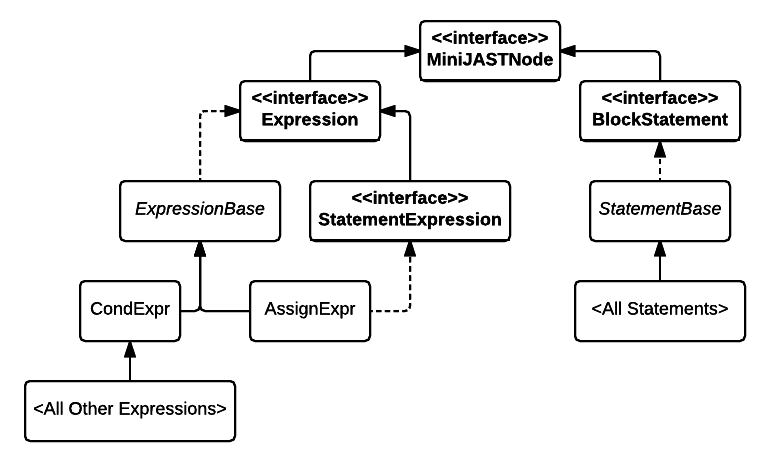
\includegraphics[width=0.8\textwidth]{TopLevelUML}
\caption{The UML diagram showing the top of the object hierarchy for \texttt{MiniJASTNode}s.}
\label{Fig:TopLevelUML}
\end{figure}

It is important to differentiate between MiniJava expressions and MiniJava statements as they must be used in different places. For example, in the production rule \texttt{WHILE~parExpression~statement} representing a \texttt{while} loop, \texttt{parExpression} may be substituted with any MiniJava expression (surrounded by parentheses), while \texttt{statement} may be substituted with any MiniJava statement. The reverse is not allowed however, meaning that \texttt{statement} may not be replaced by a MiniJava expression and vice versa. This distinction is made by the interfaces \texttt{Expression} and \texttt{Statement} (which all MiniJava expressions and statements implement respectively), and the abstract classes \texttt{ExpressionBase} and \texttt{StatementBase} (which all MiniJava expressions and statements extend respectively). 

Both interfaces and abstract classes are used here because of the need to include blanks in the grammar. There are two classes representing blanks: \texttt{FillableBlankExpr} and \texttt{FillableBlankStmnt}. The first of these should be a MiniJava expression and the second should be a MiniJava statement, meaning they should extend \texttt{ExpressionBase} and \texttt{StatementBase} respectively, but both of them must also extend the abstract class \texttt{FillableBlank}, as shown in Figure \ref{Fig:BlanksUML}. 

\begin{figure}[h]
\centering
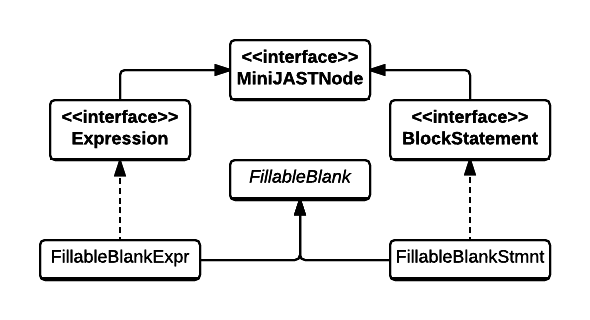
\includegraphics[width=0.8\textwidth]{BlanksUML}
\caption{The UML diagram showing how blanks fit into the object hierarchy, motivating the need for both abstract classes and interfaces to distinguish between expressions and statements.}
\label{Fig:BlanksUML}
\end{figure}

Since classes in Java cannot extend more than one base class, the only alternative is for them to implement the \texttt{Expression} and \texttt{Statement} interfaces. However, removing \texttt{ExpressionBase} and \texttt{StatementBase} would result in too much repeated code across the whole grammar, so the grammar requires both the interfaces and the abstract classes.

As important as the distinction between expressions and statements is, there do exist some expressions that can be used like statements. For an example, the MiniJava code \texttt{i~=~5;} is a statement because it ends in a semicolon,~``\texttt{;}'', but this statement consists entirely of the expression \texttt{i~=~5} (this allows for the chaining of assignments found in the Java grammar \cite[p.589]{Java8}). This sort of expression within a statement construct is not possible with all expressions, for example the code \texttt{i~+~4;} would not be valid MiniJava. To make the distinction between expressions which may be used in statements like this and those which may not, I made the interface \texttt{StatementExpression}, again, shown in Figure \ref{Fig:TopLevelUML}. This interface is only implemented by those expressions which can be used in a statement this way.

\subsection{Implementing operator precedence and associativity}

A feature of MiniJava is the concept of operator precedence, which is used to disambiguate an otherwise ambiguous grammar of expressions. Without the concept of operator precedence, the code \texttt{1~+~2~*~3} is ambiguous, as it can be read as either \texttt{(1~+~2)~*~3} which equates to 9, or as \texttt{1~+~(2~*~3)} which equates to 7. Since a single arithmetic expression cannot have more than one value, a decision must be made as to which of these interpretations is declared valid. The decision taken aligns with the standard arithmetic order of operations, such that the answer of 7 is the correct answer in this case. This example demonstrates that the multiplication operator, ``\texttt{*}'', has a higher precedence than the addition operator, ``\texttt{+}''. All the possible operators in MiniJava are found within this precedence hierarchy, and I needed some way to encode this. The method I chose for this is the natural choice, since it is suggested by the Java grammar itself \cite[p.723]{Java8}. The production rule for \texttt{AdditiveExpression} is as follows:
\begin{Verbatim}[samepage=true]
AdditiveExpression:
    MultiplicativeExpression                        (1)
    AdditiveExpression + MultiplicativeExpression   (2)
    AdditiveExpression - MultiplicativeExpression   (3)
\end{Verbatim}
and the production rule for \texttt{MultiplicativeExpression} is as follows:
\begin{Verbatim}[samepage=true]
MultiplicativeExpression:
    UnaryExpression
    MultiplicativeExpression * UnaryExpression
    MultiplicativeExpression / UnaryExpression 
    // Note that the modulus operator, %, was removed from MiniJava
\end{Verbatim}
This means that for any expression $A$\texttt{ + }$B$, the expression $A$ must only contain subexpressions that use operators with precedence at least as high as \texttt{+} and \texttt{-}, and $B$ must only contain subexpressions that use operators with precedence higher than \texttt{+} and \texttt{-}. For any expression $A$\texttt{ * }$B$, neither $A$ nor $B$ can contain subexpressions that use operators with precedence lower than \texttt{*} and \texttt{/}. This in turn indicates that an expression such as \texttt{1~+~2~*~3~+~4} can only be interpreted as \texttt{1~+~(2~*~3)~+~4}, and an expression such as \texttt{1~*~2~+~3~*~4} can only be interpreted as \texttt{(1~*~2)~+~(3~*~4)}. I wanted an operator precedence for MiniJava that is hardcoded within the grammar of MiniJava itself, just as the operator precedence of Java is hardcoded within the grammar of Java. The production rules for Java shown above suggest a natural implementation of the class that represents addition expressions:
\begin{Verbatim}[samepage=true]
class AddExpr {
    ...
    private AddExpr leftSide;
    private MultExpr rightSide;
    ...
}
\end{Verbatim}
Here, \texttt{leftSide} and \texttt{rightSide} store the left and right operands of the expression, and \texttt{MultExpr} is the class representing multiplication expressions. What has been implemented so far encapsulates parts (2) and (3) of the \texttt{AdditiveExpression} production rule above, but not part (1). This part is encapsulated by making the class \texttt{MultExpr} extend the class \texttt{AddExpr}, such that an instance of \texttt{MultExpr} may always be used in place of an instance of \texttt{AddExpr}. Note that since multiplication operators are higher in the operator precedence hierarchy, their representations are lower in the object hierarchy. This then is the solution to the operator precedence problem: to enforce an operator precedence hierarchy, first enforce an inverse object hierarchy in their representative classes, and then choose the type of each expression's operands to match the relevant terminal symbols in the relevant production rule.\footnote{Note that if you were to look at my implementation of \texttt{AddExpr}, \texttt{leftSide} and \texttt{rightSide} would both be \texttt{int}s, not \texttt{AddExpr} and \texttt{MultExpr} instances. The reason behind this is explained in section \ref{Sec:Blanks}.}

Note also that as a side-effect of this implementation, the ambiguous code \texttt{1~+~2~+~3} also only has one possible interpretation, namely \texttt{(1~+~2)~+~3}. This follows the established rules of operator associativity, which are now also hardcoded into the grammar.

\subsection{Expression types}

In MiniJava, every expression has a type which consists of a primitive type and may or may not be an array type. There are four possible primitive types: \texttt{boolean}, \texttt{char}, \texttt{int}, and \texttt{double}. The primitive types are represented in the grammar by the enumeration, \texttt{PrimType}. The type of an expression then is represented by the class \texttt{Type}, an instance of which stores the appropriate \texttt{PrimType} value and a flag determining whether or not it is an array type. These \texttt{Type}s are used by the interpreter to determine whether or not variables can contain certain values, and whether operators are being supplied with the appropriate operands.

\subsection{Blanks in code}

What distinguishes MiniJava from other languages is that the concept of a blank, a missing piece of code, is built into the grammar itself. Representations of blanks in code should enable a user to fill one with their own code. To do this programmatically, it is necessary for representations of blanks to each come with a unique id, such that users can choose which blank they are filling and the blank be searchable within the AST representing the program. The abstract class \texttt{FillableBlank} implements this functionality.The two concrete classes that extend \texttt{FillableBlank} are \texttt{FillableBlankExpr} and \texttt{FillableBlankStmnt}. The first of these can be used to replace a MiniJava expression (and thus implements the \texttt{Expression} interface so that it can be stored in a MiniJava AST), and the second can replace a MiniJava statement (and thus implements \texttt{Statement}). \texttt{FillableBlankExpr} stores an \texttt{Expression} field, \texttt{studentExpr}, which, if not \texttt{null} is representative of the code with which a user has filled the blank. Similarly, \texttt{FillableBlankStmnt} stores an \texttt{Statement} field, \texttt{studentStmnt}.\\

In this section I have described the implementation of my MiniJava language.

\section{Interpreting the language}
\label{Sec:Interpret}

In this section I explain how MiniJava programs are interpreted.

To correctly interpret MiniJava, several requirements must be met by the interpreter:
\begin{enumerate}
\item{The scope of variables must be handled, such that when a variable is used its current value can be accessed, and the same variable can't be declared twice in one scope.}
\item{Expressions must be able to propagate their values upwards, so that surrounding expressions and statements can use them.}
\item{Flow control must be handled, such that break and continue statements can be used in loops.}
\item{If an exception is raised during execution, the exception should propagate up and halt execution, preferably delivering a useful message.}
\end{enumerate}

\subsection{Handling scope}

The scope of variables is handled by the interpreter with instances of the \texttt{Context} class. Part of its definition is shown below:
\begin{Verbatim}[samepage=true]
public class Context {
    public Stack<HashMap<String, Type>> namesToTypes;
    public Stack<HashMap<String, Object>> namesToValues;
    ...
}
\end{Verbatim}
The \texttt{namesToTypes} field is a stack of maps from names (as \texttt{String} values) to instances of my \texttt{Type} class. Every variable that is declared in this scope will have an entry in the map on top of this stack, recording the type of that variable. The \texttt{namesToValues} field is a stack of maps from names to instances of \texttt{Object}. If a variable has an entry in the map on top of this stack, then, in this scope, the variable has the value stored under it in the map. It is possible for a variable to have an entry in the map on top of the \texttt{namesToTypes} stack, but not in the map on top of the \texttt{namesToValues} stack: this indicates that the variable has been declared but not initialised in this scope.

During execution, the interpreter must keep track when variables will go out of scope. This is handled by the \texttt{stepIn} and \texttt{stepOut} methods in \texttt{StatementBase}. The \texttt{stepIn} method is called whenever execution enters a new, deeper, scope. This method copies every key value pair in the maps on top of their respective stacks into new maps, and pushes these new maps onto the stack. Thus every entry in one of the stacks represents a different scope: as you move down the stack, you move outward through the nested scope. The \texttt{stepOut} method is called whenever execution leaves the current scope. Pseudocode for this method is shown below:
\begin{Verbatim}[samepage=true, tabsize=4]
void stepOut(Context c) {
	if (the stacks have size 1)
		return; // This keeps the outer level of scope available for 
		        // solution validation

	pop both stacks in c, store top of namesToValues stack in oldMap
	for (name n in keys of oldMap)
		if (n is key of new top of namesToTypes)
			set the value stored with n in the new top of namesToValues 
			to be the same as that in oldMap
}
\end{Verbatim}

At this point, all the variables that do not exist in the new scope should be forgotten, and every variable that does exist in this new scope should have their value updated to the value it was in the old scope. The \texttt{stepOut} method does this by popping the top off both stacks, and writing back the values of variables that are still in scope.

\subsection{Propagating expression values}

Consider the expression \texttt{(2*3)+4}. In MiniJava, this expression might be represented by an \texttt{AddExpr} storing a literal with the value \texttt{4} as the right operand, and a \texttt{MultExpr} as the left operand. This \texttt{MultExr} would store literals with values \texttt{2} and \texttt{3} as the left and right operands. During the evaluation of an expression, the most deeply nested parts of the expression must be evaluated first, so that their values can be used further up. There is no point trying to evaluate the \texttt{AddExpr} before we know the value of \texttt{(2*3)}. Thus, the \texttt{MultExpr} needs a way to communicate to the \texttt{AddExpr} that it has a value of \texttt{6}, so that the \texttt{AddExpr} can be evaluated to \texttt{10}. Likewise, whatever context the \texttt{AddExpr} is in needs to be told it has the value \texttt{10}. The way this is done in MiniJava is using implementations of the \texttt{ReturnValues} abstract class. This class represents the notion that some value is being returned by an expression, but allows any type of value to be returned, no matter what primitive type the value takes, and whether it is an array or not. To return a value of a particular primitive type, the appropriate one of these four implementations must be used: \texttt{ReturnValuesBool}, \texttt{ReturnValuesChar}, \texttt{ReturnValuesInt}, or \texttt{ReturnValuesDouble}. Each of these stores a value of the appropriate type. If an array value is being returned by an expression, then a further implementation of \texttt{ReturnValues} must be used, the generic class \texttt{ReturnValuesArray<T>}. This class makes use of Java Generics as it stores an internal \texttt{ArrayList<T>} of values.

\subsection{Control flow}

In the same way that MiniJava expressions dispense values, MiniJava statements dispense control flow commands. These commands can be to ``break'', to ``continue'', to ``return'', or there can be no command, in which case execution continues as normal. The MiniJava interpreter represents these commands using the \texttt{FlowControl} enumeration, which has the four values \texttt{BREAK}, \texttt{CONTINUE}, \texttt{RETURN}, and \texttt{NONE}. Whenever a statement is executed, the interpreter looks for which value is dispensed and reacts accordingly. 

\subsection{Handling exceptions}

Several custom exceptions are used by the interpreter, to differentiate between when an error occurs in the MiniJava program being interpreted, and when an error occurs in the interpreter itself. All these custom exceptions subclass the base class of \texttt{MiniJavaException}, and the majority of them are analogous to standard Java exceptions. For example, the \texttt{OutOfBoundsException} is thrown by the interpreter whenever an index is used in an array where no such index exists. This exception is analogous to Java's \texttt{IndexOutOfBoundsException}.

\subsection{The interpreter itself}

The MiniJava interpreter is implemented using the \texttt{evaluate} method in the \texttt{Expression} interface, and the \texttt{execute} method in the \texttt{Statement} interface. The method signatures of these two methods are shown below:
\begin{Verbatim}[samepage=true]
public interface Expression extends MiniJASTNode {
    ReturnValues evaluate(Context c) throws MiniJASTException;
    ...
}

public interface Statement extends MiniJASTNode {
    FlowControl execute(Context c) throws MiniJASTException;
    ...
}
\end{Verbatim}
It can be seen that the interpreter makes use of all the components meeting the requirements for the interpreter. The \texttt{evaluate} method is overridden by every class representing a MiniJava expression, and the \texttt{execute} method is overridden by every class representing a MiniJava statement. This means that both methods are recursive: expressions being evaluated will call the \texttt{evaluate} method on their subexpressions for example. Typically, execution is initiated with an empty \texttt{Context} object that becomes more populated as more variables are declared. 

It is important to remember that the MiniJava grammar also contains the notion of blanks in code, and thus the interpreter must be equipped to deal with these appropriately. If a blank has not yet been filled, then the interpreter should throw a custom exception, but if the blank has been filled, then execution must continue as if there was no blank there. The \texttt{FillableBlankExpr} and \texttt{FillableBlankStmnt} classes override the \texttt{evaluate} and \texttt{execute} to implement this functionality. This is shown for \texttt{FillableBlankExpr} below, but \texttt{FillableBlankStmnt} is exactly analogous.
\begin{Verbatim}[samepage=true, tabsize=4]
ReturnValues FillableBlankExpr::evaluate(Context c) throws ...{
	if (the blank is not filled)
		throw BlankEmptyException;
		
	return the result of evaluating the stored expression with c.
}
\end{Verbatim}

In this section I explained how MiniJava is interpreted.

\section{Representing questions and solutions}
\label{Sec:Q&A}

In this section I explain how exercises are represented using the \texttt{AbstractPExercise} class, and give an example of how a specific exercise can be encoded by extending this class.

When presented to a student learning a programming language, an exercise can be broken up into the following components:
\begin{itemize}
\item{The question, telling the student what they are expected to do.}
\item{A model solution to the problem presented with parts of the code left blank for students to fill in.}
\end{itemize}

Following these guidelines, a representation of a programming question should be capable of the following:
\begin{enumerate}
\item{Adding and removing blanks from the model solution to make the problem harder or easier.}
\item{Filling those blanks with MiniJava representations of student submitted code.}
\item{Checking that the problem is solved by the provided solution.}
\end{enumerate}

The abstract class \texttt{AbstractPExercise} provides the framework for classes extending it to fulfil all these requirements. I explain how the points above are addressed by \texttt{AbstractPExercise} in order.

\subsubsection*{1. Adding and removing blanks from the solution}

The algorithms used to add and remove blanks from the solution code are complex enough to warrant a dedicated section, and are thus discussed in Section \ref{Sec:Blanks}.

\subsubsection*{2. Filling blanks with student submitted code}

Since representations of blanks in code have their own unique identifier, the blank that a user wishes to fill can be selected using it. To fill a blank with the representation of a user's code, the representation of the blank itself must be found within the program's AST, before the representation of the code is stored within it. This is done using a depth-first-search through the AST to find blanks which, when found, have their identifiers compared with the target identifier. If they do not match, then the search moves on. If they do match, then the blank is filled with the student's code. If the search fails, then it can be reported that no blank with the suggested identifier exists within the solution.

\subsubsection*{3. Checking that the problem is solved by the provided solution}

There are two possible ways of checking whether a solution is valid: either the value of a variable can be compared with a target value, or the result of a print statement can be inspected. The first of these approaches requires an \texttt{Id} field to be declared in the concrete class representing the problem, assigned the appropriate name in the constructor. Once the solution has been executed, the final value of this variable can be accessed by evaluating the \texttt{Id} with the \texttt{Context} object used during execution. In contrast, the second approach can be implemented by checking the contents of the file written to by the representation of the print statement. 

\subsection{An example exercise}

An example concrete class extending \texttt{AbstractPExercise} is \texttt{FactorialExercise}, which represents an exercise in which the student is asked to use a \texttt{while} loop to calculate the factorial of a random integer $N$, storing the result in the variable \texttt{total}. The model solution code is shown below:
\begin{Verbatim}[samepage=true]
int total = 1, n = N;
while (n > 1) {
    total *= n--;
}
\end{Verbatim}
This code calculates $N\times(N-1)\times\dotsb\times2\times1=N!$  and stores it in \texttt{total} as required. In the \texttt{FactorialExercise} constructor, the value of $N!$ is calculated in the same way and stored, and a field of type \texttt{Id} is set up with the name ``\texttt{total}''. To check a solution, the class runs the solution, evaluates \texttt{totalID} with the appropriate \texttt{Context} object, and compares its final value with the correct answer stored previously, returning \texttt{true} if they are the same and \texttt{false} otherwise.

In this section I have presented the class \texttt{AbstractPExercise}, shown how it fulfils the requirements for representing an exercise, and shown a concrete example that extends it.

\section{Adding and removing blanks}
\label{Sec:Blanks}

This section describes first the algorithm that adds a blank to a MiniJava program that can later be filled in by a student, followed by the algorithm that replaces a blank with the original code snippet.

\subsection{Choosing the algorithm for adding blanks}

The difficulty of a problem is based on the difficulty of the question itself and the percentage of the model solution that is blank when it is presented. Changing the question itself can be considered a coarse-grained adjustment to the problem's overall difficulty, while changing the percentage of the model solution that is blank is a much more fine-grained adjustment of overall difficulty. When we wish to adjust the difficulty of the problem, we would prefer to have the greatest control over the difficulty possible, able to make the finest-grained adjustments. For this reason, the algorithm that chooses which node in a model solution to replace with a blank should make the choice that causes the smallest growth in the percentage of the whole that is blank. Additionally, we would prefer to distribute these blanks across the whole solution, rather than concentrating them in any one part. 

\begin{wrapfigure}{r}{0.3\textwidth}
  \centering
    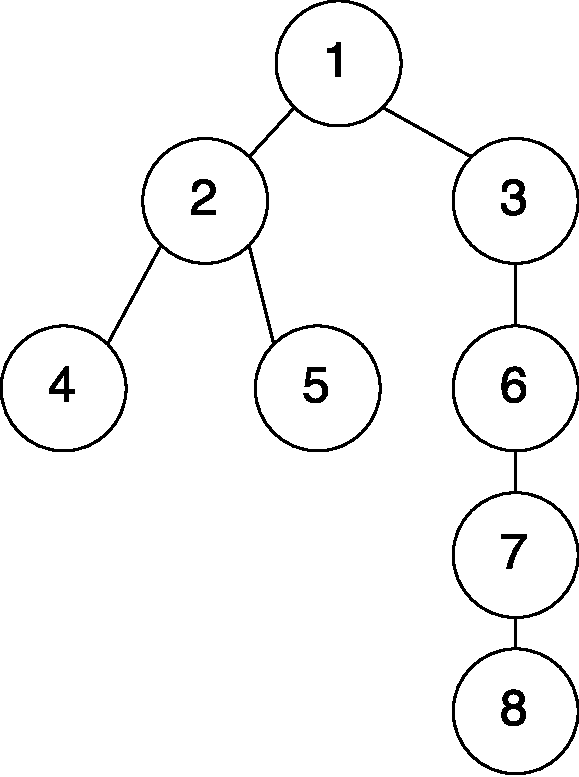
\includegraphics[width=0.28\textwidth]{ExampleTree}
  \caption{An example of an AST with nodes labeled for clarity.}
  \label{Fig:Tree}
\end{wrapfigure}

Figure \ref{Fig:Tree} shows an example AST, with its nodes numbered for reference. Using this tree we can compare different algorithms for selecting nodes, and see which best fulfils our requirements. Since we want to be able to add blanks to the model solution until the entire solution is blank, we should consider traversal algorithms. The algorithm will terminate when a node is selected to be made blank, and when it is next run it should (effectively) pick up from the same point. Since, clearly, the first choice of node to be replaced should be a leaf (any other choice would cause a larger percentage increase of the number of blank nodes, since such a node would have children that would simultaneously be made blank), some standard algorithms suggest themselves. The Depth First Traversal algorithm, when run on the example tree, would produce the output: 4,~5,~2,~8,~7,~6,~3,~1. Notice that node 2 is visited before node 8. This algorithm would concentrate all the blanks in the left hand side of the tree, reaching up to the left-most child of the root before considering the right hand side of the tree. This renders the Depth First Traversal algorithm unfit for our purposes. Another potential traversal algorithm to consider is the Reverse Level Order Traversal algorithm, which acts something like a Breadth First Traversal from the leaves upwards. When run on the example tree, this algorithm would produce the output: 8,~7,~4,~5,~6,~2,~3,~1. This algorithm suffers from a similar problem: node 7 is visited before node 4. This results in the blanks being concentrated on areas of the tree that have the deepest nodes, neglecting all other areas. This again means that the Reverse Level Order Traversal algorithm is not fit for our purposes. The ideal output for our algorithm would be as follows: 4,~5,~8,~2,~7,~6,~3,~1. This does a good job of distributing blanks across the tree without reaching the upper levels of the tree too soon. Since the tree is unbalanced, once we have visited node 2 we have no choice but to visit the long chain of nodes on the right hand side of the tree, but at least there are a decent number of blanks on both sides of the tree at that point. This output can be attained by a traversal algorithm that operates as described below, but before that it is worth making a somewhat subtle clarification. When describing these algorithms it has been useful to think of them as traversal algorithms, even though I would not be using them that way. At each execution of the algorithm, a single node is made blank. On the next execution, a different node will be made blank. After a finite number of executions, the entire solution will be blank. Since every node is selected exactly once, the combination of all the executions leading to an empty model solution can be considered a traversal of the tree. The following algorithm is difficult to describe as a simple traversal, since that is not its aim. As such, the following description includes directions to remove nodes from the tree, something that you definitely wouldn't find in a standard traversal. The simplest description of this algorithm comes with the appreciation that the purpose of the algorithm is in fact to replace nodes with blanks\footnote{Replacing a node with a blank is similar enough to deleting the node entirely that they can be interchangeable in this context. This is explained in the following paragraphs.}, not traverse the tree. With that in mind, here is a description of the ideal ``traversal'' algorithm:

\begin{enumerate}
\item{Traverse the tree as in the Depth First Traversal algorithm.}
\item{Whenever a leaf is reached, return that node, and remove it from the tree.}
\item{Repeat until the root has been removed.}
\end{enumerate}

It can be seen that this algorithm does indeed produce the desired output, 4,~5,~8,~2,~7,~6,~3,~1. During the first pass of the tree, the leaves labeled 4, 5, and 8 are returned and removed. Removing these leaves means that nodes 2 and 7 are now the leaves of the tree. On the next pass through, these leaves are returned and removed. The ``tree'' is now a simple chain of the nodes (returned in the order of bottom to top) 6, 3, 1.

\subsection{Adding a blank}

The problem my algorithm must solve is more complex than a simple traversal. Not only should my algorithm terminate mid-traversal and be able to pick up from that point at the start of the next execution, but the process of actually inserting a blank into the tree is non-trivial. On top of that, the results of executing the algorithm have to be reversed in order to replace a blank with the original code snippet. 

Since the first step is to traverse the tree as a Depth First Traversal, we must first implement this, using a \texttt{Stack<MiniJASTNode>} to store the nodes that still need to be dealt with. We start by pushing the root node (found in the \texttt{solution} field of the \texttt{AbstractPExercise} class) on to the nodes stack, as usual, and as usual we process this node before adding its children to the stack. Point 2 of the algorithm description says that when we find a leaf, we remove it from the tree. In the actual algorithm we wish to replace the node with a blank (the process for which I explain shortly), but since we are do not actually remove the node from the tree, we have a problem. Once we have made all the leaves of the tree blank, we have no more leaves to choose; this is in direct contrast to when we were simply removing leaves thereby creating more leaves. To fix this problem, we redefine the concept of leaves: a node is a leaf it has no children or all of its children are blank. In this way, by making leaves blank we are in fact creating more leaves.

When we find a leaf, we wish to replace it with a blank. To do this, we have to replace the reference to the node in its parent with a reference to a new blank. At the moment, you cannot index nodes: you cannot access the $n$th child of a node, since they are simply stored in \texttt{private} fields. This means that it is very difficult to replace the reference to a child within a parent, without implementing a setter in every class that could translate the integer index to the appropriate field. This seems a lot more tiresome than simply allowing one to index nodes. To enable this, rather than store their children directly as fields, each class in the implementation stores all its children in an array and separately stores indices into the array to provide access to the children. When we wish to replace a node with a blank, we store a blank at the appropriate index within its parent's array of children. This means that we need to keep track of what the parent of the current node is, and also of the current node's index within its parents.

Since we need to be able to undo the effects of an execution of the algorithm to be able to restore the original code, we need to store the nodes that were replaced as well as the list of indices giving the path through the tree to each node's original location. These are stored in \texttt{Stack}s in the  \texttt{AbstractPExercise} class. The indices are also useful in enabling us to restart the algorithm where it left off. At the beginning of the algorithm, we take the top of the stack of indices and follow them through the tree to where the last node was made blank, and then continue the traversal. 

\subsection{Removing a blank}

In contrast to adding a blank, the algorithm that removes a blank from the model solution is much simpler. We simply take the top off the stack of replaced nodes and the stack of indices, follow the indices to the parent of the specific node, and use the last index to reinsert the node back in to its parent.

This section described the implementation of the algorithms that introduce blanks to and remove them from a MiniJava program.

\section{The \texttt{ExerciseSetter}}
\label{Sec:ExSet}

In this section I describe how I made use of the language and its features to design the \texttt{ExerciseSetter} class, which can set exercises and adjust their difficulty.

The intuition behind the design of the \texttt{ExerciseSetter} comes from the imagined use case of students in a class where the student to teacher ratio is very high, and students may not have instant access to a teacher in the case that they find the presented exercises too easy or too difficult. The challenge in this scenario would be to programmatically detect that the student's capability is not matched with the difficulty of the exercise, and to present an easier or a harder problem appropriately. The \texttt{ExerciseSetter} facilitates this by implementing a very simple performance heuristic and by storing several questions of various difficulties, such that ideally all students could be catered too. Using the performance heuristic, the \texttt{ExerciseSetter} attempts to adjust the current problem's difficulty appropriately.

The performance heuristic operates on the assumption that the performance of the students can be inferred from the number of attempts at solving the problem before their solution was correct, and the comparison between the number of nodes in the model solution tree and the number of nodes in the student's solution tree. The more attempts a student required to solve the problem correctly, the more difficult they found the problem. Also, if a student used many more nodes to solve the problem than the model solution did, then it is likely that they haven't understood a core concept being tested: they may have unnecessarily unrolled a loop for example. 

If, once an exercise has been solved, the next exercise needs to be harder, according to the performance heuristic, then the \texttt{ExerciseSetter} should add blanks to the solution until either the exercise is hard enough, or the entire solution is blank. If the latter occurs, then the \texttt{ExerciseSetter} should attempt to present a harder question, with enough of the solution blank that the answer is not given to the student at first glance. If instead the exercise needs to be easier, then the \texttt{ExerciseSetter} should remove blanks from the solution until either the exercise is easy enough, or there are no blanks in the solution. If the latter occurs, then the \texttt{ExerciseSetter} should attempt to present an easier question.

In this section I have detailed the implementation of the \texttt{ExerciseSetter}.

\section{Extension: the parser}
\label{Sec:Parsing}

In this section I explain how a parser for MiniJava was implemented as an extension using the ANTLR parser generator\cite{ANTLR4}, and how a representation of an input MiniJava program can be built using it.

The parser grammar (which can be found in Appendix \ref{App:Parser}) is based on an existing ANTLR parser grammar for Java\footnote{https://github.com/antlr/grammars-v4/tree/master/java - last accessed May 13th}. It would not have been worthwhile for me to write an entire grammar from scratch when there was such a readily available alternative. It is always good to use existing libraries or tools if they are available. 

The ANTLR tool generates recursive descent parsers from input grammars. The typical usage of ANTLR follows this process:
\begin{enumerate}
\item{Write a grammar in a grammar file.}
\item{Run the ANTLR tool on this grammar file to generate a parser.}
\item{When this parser is executed with input source code, ANTLR's internal representation of the corresponding parse tree is built.}
\item{Using either a ``listener'' or a ``visitor'', walk the generated parse tree, taking actions at each node, processing the source code as desired.}
\end{enumerate}
The following code shows how to build a MiniJava representation for the source code \texttt{i~=~4;}.
\begin{Verbatim}[samepage=true, numbers=left]
AssignExpr aE = new AssignExpr();
Id i = new Id();
i.setUpId("i");
Literal four = new Literal();
four.setUpLiteral(PrimType.INT, "4");
aE.setUpAssignExpr(i, AssignOp.EQ, four);
ExpressionStmnt eS = new ExpressionStmnt(aE);
\end{Verbatim}
Considering this representation as a parse tree, this can be seen as line 0 (i.e. the invisible line before line 1) visiting the \texttt{ExpressionStmnt} node and visiting its only child, the \texttt{AssignExpr} node in line 1. This node's first child is visited in lines 2 and 3, and its second child is visited in lines 4 and 5. Once all the children of the \texttt{AssignExpr} have been visited, the instance itself can be set up on line 6. Once all the \texttt{ExpressionStmnt}'s children have been visited, its instance can be set up on line 7. This example demonstrates that in general, program representations are generated by recursively visiting each expression or statement's children, in a similar way to how a program representation is interpreted.

By default, the ANTLR tool generates a listener interface and base class along with the parser. A listener is characterised by providing callback methods that are triggered by an automatic parse tree walker: listener methods don't have to explicitly visit their children. A visitor on the other hand gives the user more control over the walk, requiring explicit commands to visit the children of each node. While this means that it takes less work to use a listener (as the parse tree walker is already built in), the visitor paradigm is more appropriate for building my library's representation of the MiniJava source code. While the listener methods all return \texttt{void}, requiring the instances representing the children nodes to be stored somewhere in memory prior to setting up the current node, the base visitor, \texttt{MiniJavaBaseVisitor<T>}, is generic, with methods returning a \texttt{T} object. This means that the visitor methods can be made to return \texttt{MiniJASTNode}s, which can be cast to \texttt{Expression}s or \texttt{Statement}s as appropriate (as shown in Figure \ref{Fig:TopLevelUML} on page \pageref{Fig:TopLevelUML}). By using a visitor rather than a listener, I was able to more closely imitate the way that program representations are build in code (shown above). My visitor implementation can be found in \texttt{MiniJavaASTBuilder}, a class which extends the \texttt{MiniJavaBaseVisitor<MiniJASTNode>} class supplied by the ANTLR tool.

\subsection{Challenges when parsing}

Java, and by extension MiniJava, is a language that suffers from the ``dangling-else'' problem: a particular problem arising from an ambiguous grammar. Consider the MiniJava code shown below:
\begin{Verbatim}[samepage=true,tabsize=4]
if (i == true)		 (1)
	if (j == false)	(2)
		k = 1;
else
	k = 2;
\end{Verbatim}
A parser could not make a decision as to whether the \texttt{else} statement ``belongs'' to the first or the second \texttt{if} statement. Since the grammar is ambiguous, a decision must be made for the parser. The decision taken in Java\cite[p.417]{Java8}, and thus in MiniJava, is to attach the \texttt{else} statement to most inner \texttt{if} statement possible (which in the example above would be the one labeled \texttt{(2)}, even though the indentation may suggest that the programmer intended it to be the one labeled \texttt{(1)}). To implement this decision, the grammar distinguishes between \texttt{Statement}s and \texttt{StatementNSI}s (where NSI stands for ``No Short If'', i.e. there are no \texttt{if}s without associated \texttt{else}s). The way this solves the problem becomes apparent on inspection of the following rules in the grammar (presented in context in Appendix \ref{App:Parser}):
\begin{Verbatim}[samepage=true, tabsize=4]
statement:
	...
	| IF parExpression statement 				
	| IF parExpression statementNSI ELSE statement	  
	...
	;
	
statementNSI:
	...
	| IF parExpression statementNSI ELSE statementNSI
	...
	;
\end{Verbatim}
The \texttt{statement} rule gives productions for both a short \texttt{if} (i.e. with no attached \texttt{else}) and a long \texttt{if}, while the \texttt{statementNSI} rule only produces a long \texttt{if}. It can be seen that using these rules to parse the code above will reach a dead end if the first \texttt{if} statement is parsed as a long \texttt{if}, since its first sub-statement would have to be a \texttt{statementNSI}, and this rule has no viable way of parsing the second \texttt{if} statement. 

Another problem encountered while writing the parser can be discovered on inspection of the local variable declaration production shown below:
\begin{Verbatim}[samepage=true, tabsize=4]
blockStatement: 
	primitiveType variableDeclarators SEMI	# localVariableDeclaration
	...
	;
\end{Verbatim}
This production is used in the creation of \texttt{LocalVarDec} instances, which require the appropriate \texttt{PrimType} to set up correctly. As the visitor arrives at a node produced like this in the parse tree (by calling the \texttt{visitLocalVariableDeclaration} method found in \texttt{MiniJavaASTBuilder}) it needs to visit the node's children in order to gather the necessary objects to set up the \texttt{LocalVarDec} object. Since visitor methods return \texttt{MiniJASTNode}s, the \texttt{visitPrimitiveType} method (also found in \texttt{MiniJavaASTBuilder}) needs to return an object whose class implements \texttt{MiniJASTNode} and represents a primitive type. Until this point, no such class existed. The enumeration \texttt{PrimType} does not implement \texttt{MiniJASTNode}, as that would require overriding all the methods declared in the interface separately for each value, as they are in \texttt{SingleWordStmnt}. Since this would be a lot of wasted code, I instead wrote a new class, \texttt{PrimTypeCarrier}, for precisely this purpose. This class implements \texttt{MiniJASTNode} and has a public field of type \texttt{PrimType}, meaning it only needs to implement (trivially) all of the interface methods once. An instance of this class can thus be created in the \texttt{visitPrimitiveType} method (setting the \texttt{PrimType} field value appropriately), which can then be returned to the \texttt{visitLocalVariableDeclaration} method for setting up the \texttt{LocalVarDec} object.

\subsection{Using the parser}

The \texttt{ExerciseSetter} class provides an interface through which students may fill blanks by submitting their own code as a \texttt{String}. To get the representation of this code to actually fill the blank, of course the parser must be used, but this presents an interesting problem. Certain code snippets have the potential to be both \texttt{Expression}s and \texttt{Statement}s. An example of this is the code snippet \texttt{total = 1}. This can be parsed as an assignment, and would thus be classed an \texttt{Expression}, or a variable declaration, where the surrounding context might be \texttt{int total = 1;}, which would categorise this snippet as a \texttt{Statement}. Fortunately the parser  has a solution to this, as the starting terminal symbol for the grammar is not fixed. The \texttt{ExerciseSetter} can check whether the blank being filled represents an \texttt{Expression} or a \texttt{Statement}, and then sets the entry point of the parser to be either \texttt{expression} or \texttt{blockStatement} appropriately.\\

In this section I have described how the ANTLR parser generator can be used to generate parsers for the MiniJava grammar, and how program representations can be built using visitors.

\section{Extension: the GUI}
\label{Sec:GUI}

In this section I describe the implementation and function of the GUI as an extension.

\begin{figure}[h]
\centering
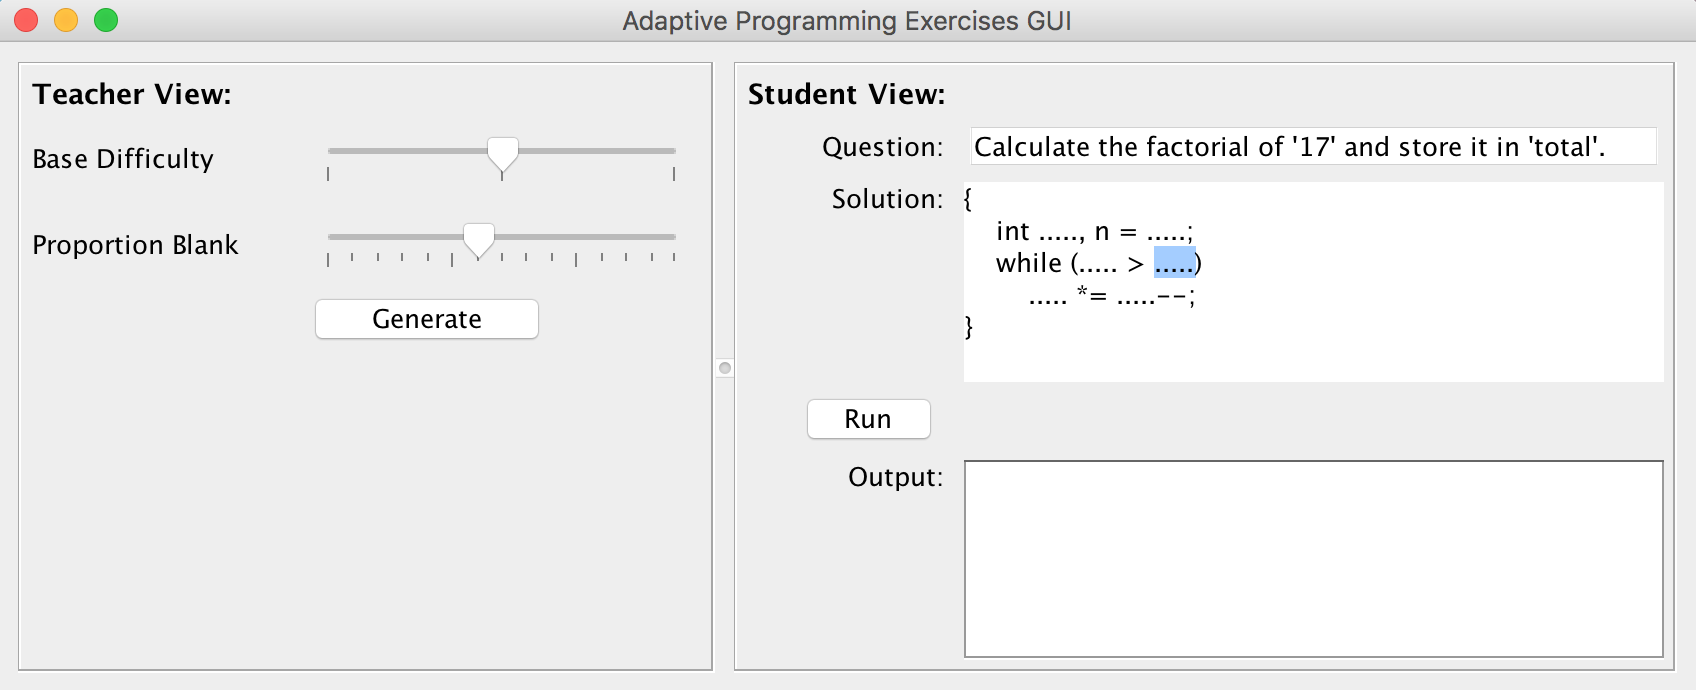
\includegraphics[width = \textwidth]{GUI}
\caption{An example screenshot taken of the GUI peripheral.}
\label{Fig:GUI}
\end{figure}

The GUI demonstrates some of the possible uses of this set of tools. It shows how a teacher might manually set the difficulty of a particular exercise and how a student could fill in the blanks and run their solution. An example screen from the GUI is shown in Fig \ref{Fig:GUI}. The top slider determines the difficulty of the question: the further to the left the slider is, the easier the question will be. The bottom slider affects the difficulty of the problem: the further it is to the left, the fewer blanks there will be and thus the easier the problem will be to solve. When the ``Generate'' button is clicked on, the corresponding exercise will be displayed on the right. 

As shown in the screenshot, the ``Solution'' box on the right is editable, allowing students to directly input their own code, filling in the blanks or otherwise. When the ``Run'' button is clicked, the code in this box is parsed and set as the solution to the exercise. This solution is then run, and the validity of the solution checked. The GUI reports whether the solution was correct or not, and attempts to present error messages in a user friendly manner if any were produced. If the solution was correct, the student's performance is measured and the difficulty of the next exercise set accordingly. Example inputs and outputs of the GUI are shown in Section \ref{Sec:GUIEval} of the Evaluation.

The GUI was designed using the IntelliJ Swing plugin\footnote{https://www.jetbrains.com/help/idea/2017.1/swing-designing-gui.html}. This plugin allowed me to drag and drop components into place on the form before programming their functionality with the adjoining bound class. The class stores a reference to an \texttt{ExerciseSetter} object, which is where all the data comes from, and where the commands from the user are delivered to.

%%%%%%%%%%%%%%%%%%%%%%%%%%%%%%%%%%%%%%%%%%%%%%%%%%%%%%%%%%%%%%%%%%%%%
% Evaluation Chapter

\chapter{Evaluation}

In this chapter I demonstrate that all of the original goals of the project were achieved. In Section \ref{Sec:Func} I show that all the components fulfil the requirements laid out in Chapter 1. The trends that emerge as the difficulty is adjusted are analysed in Section \ref{Sec:DiffTrends}, and the development process is critiqued in Section \ref{Sec:DevProc}.

\section{Correct functionality}
\label{Sec:Func}

A test suite consisting of a total of 113 tests (all of which pass when run on the current source code) demonstrates that the aims of the project are satisfied by my implementation. This section begins by describing the implementation of these tests, before evaluating the function of some of the more complex components.

\subsection{Unit tests}

Of the 113 unit tests I implemented, 84 of these test the interpreter, 14 test the parser, 12 test the exercise representations, and 3 test the \texttt{ExerciseSetter} class. The number of these tests is determined by the size of the components: although the interpreter is simple it is large, and the \texttt{ExerciseSetter} is complex but small. Each of these tests operate by setting an initial state, executing the code being tested, and comparing the final state with the expected value. 

For the interpreter for example, this means setting up one of the classes representing a syntax construct, running the interpreter on the instance, and checking that the desired outcome is seen. This outcome could be the value of an expression, the value of a variable, or some flow control command. In the case of the \texttt{ForStmnt} class (representing a \texttt{for} statement), the test sets up an instance of the class within a representation of the following code to calculate a factorial:
\begin{Verbatim}[samepage=true,tabsize=4]
int sum = 1;
for (int i = 5; i > 0; i--) {
	sum = sum * i;
}
\end{Verbatim}
The test runs the interpreter on the representation of this code and checks that the final value of \texttt{sum} is 120. The validity of this test is thus based on the correct functionality of the representations of local variable declarations, assignment expressions, relation expressions, post-decrement expressions, and multiplicative expressions.  Given this, I wrote the tests in such an order that each syntax construct was tested before it was used in any other test.

The tests for the parser on the other hand are mainly regression tests. This means that whenever a bug has been found (e.g. through use of the system) and fixed, a test looking for that specific bug has been added to the test suite, to ensure that I never accidentally reintroduced it.

\subsection{The \texttt{ExerciseSetter} class}
\label{Sec:ExSetEval}

The aim of the \texttt{ExerciseSetter} class is to be capable of measuring a student's performance and adjusting the difficulty of the following exercises appropriately.

The measurement of a student's performance is represented by a \texttt{float} value. If this value is positive then the student has performed well, if it is negative the student performed poorly. The magnitude of this value indicates the size of the adjustment necessary for the next exercise. Figure \ref{Fig:PerfGraph} shows how the measured performance depends on both the number of attempts a student has made to give a correct solution and also the number of extra nodes they used in their solution compared with that of the model solution. It shows the contours of the surface, which is a function of both variables. The orange line labelled 0 represents the zero contour. That is, any solution that maps to a point above that line (on the 2D plot) is unsatisfactory, and will result in the next exercise being easier. Solutions mapping to points below the zero contour are of an acceptable standard such that the next exercise will be harder. As a hypothetical example, say student A provided a correct solution in two attempts, using the expected number of nodes, student B required four attempts but still used the expected number of nodes, and while student C also provided a correct solution in two attempts, they used nine nodes more than necessary. As can be seen on Figure \ref{Fig:PerfGraph} only student A's solution has a performance value greater than zero.

The performance measurement varies as a function of the number of attempts squared, meaning that the difference in measured performance between two and three attempts is about one whereas the difference between four and five attempts is four. This is so that solutions that required more numerous attempts are taken as indicative of poorer performance. In my opinion, requiring multiple attempts suggests a lack of understanding of the concepts underlying the question being answered or that the student is simply guessing. I have defined the cut-off point for the number of attempts as 2.5. That is, if a student requires two attempts or fewer, the system determines that the next exercise can be harder, but if a student requires three attempts or more, the next exercise will be easier. This cut off was chosen to allow for one careless mistake before assuming lack of comprehension.

If the student uses fewer nodes than the model solution, they may either have found a more efficient solution, or they may have ``cheated'' and not used the appropriate syntax constructs being taught (e.g. found $n!$ using a calculator and simply assigned the value to the variable, rather than using the expected \texttt{while} loop). At present, when a student uses fewer nodes, the system cannot tell the difference between a student showing greater understanding and one ``cheating''. Therefore, the performance function does not take this into account, shown by the horizontal contours to the left of the $x=0$ vertical. When the number of extra nodes used is greater than zero, it is likely that the student has not understood the best way to solve the question (e.g. unrolled the while loop to calculate $n!$). For this reason, the greater the number of extra nodes used, the worse the measured performance.

During the evaluation of this system, I became aware of a possible limitation. At the moment, there is no way for a student to ``fail'' a question and no way for them to give up. This means that if a student is given a low performance score for a solution, and thus the same question but with fewer blanks, then the student has already answered this question at a greater difficulty, and this new question might feel trivial to them. Whether this is a problem is debatable: a student could find it frustrating to have to answer the same question again, or they might appreciate being shown more of the model solution if their own was very different. An alternative implementation that provides a way for a student to give up might be such that a correct solution always results in a harder question, and that an easier question is only delivered if the student is forced to give up. This new approach might fail students in another way, in that if a student is reduced to guessing and manages to guess the correct response, then that student may not have understood the underlying material and nevertheless be presented with a harder question. An area of further work might be determining which of these approaches promotes greater knowledge retention.

\begin{figure}
  \centering
    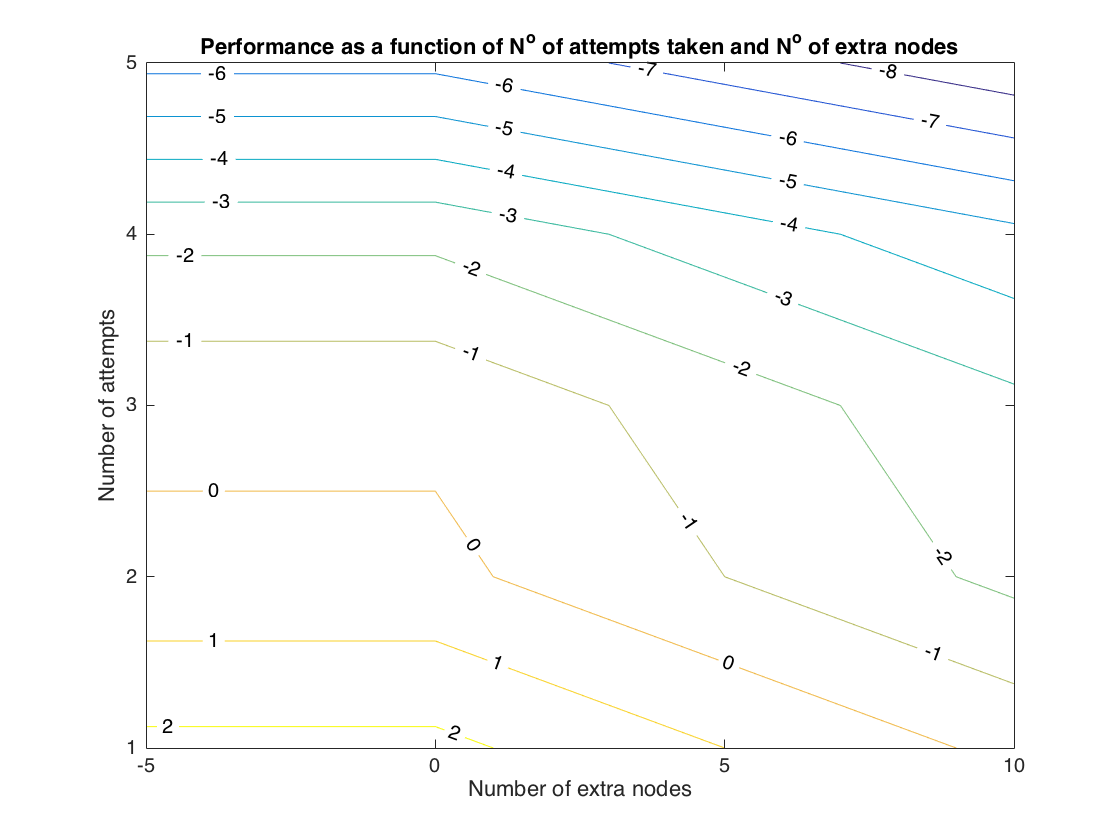
\includegraphics[width=0.8\textwidth]{PerfGraph}
  \caption{The contours of the performance surface, dependent on the number of attempts required and the number of extra nodes used. Points A, B and C show the performance measurement of three hypothetical students.}
  \label{Fig:PerfGraph}
\end{figure}

\subsection{The GUI extension}
\label{Sec:GUIEval}

The GUI brings together all of the components and provides an interface for users. The screenshots in Figure \ref{Fig:GoodGUIScreens} show the output given when a student solves the exercise in the best way possible, that is in one attempt and with no more nodes than expected.

\begin{figure}
\centering
  \begin{subfigure}{.45\textwidth}
    \centering
    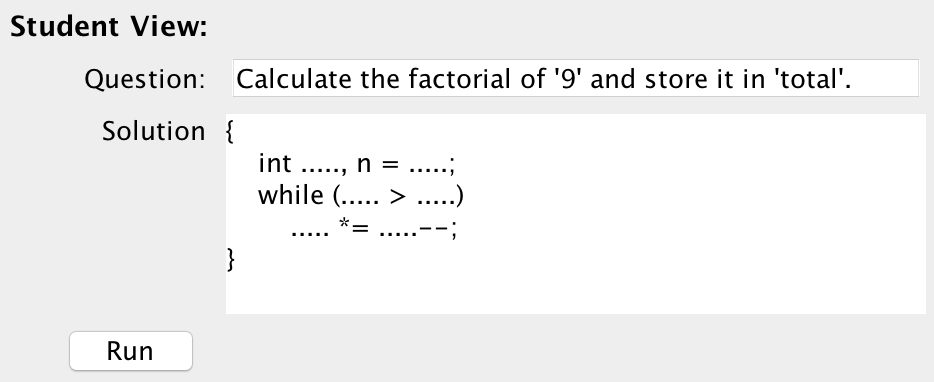
\includegraphics[width=.9\linewidth]{InitialQuestion}
    \caption{The initial question presented to the student.}
    \label{SFig:GGS1}
  \end{subfigure}%
  \;
  \begin{subfigure}{.45\textwidth}
    \centering
    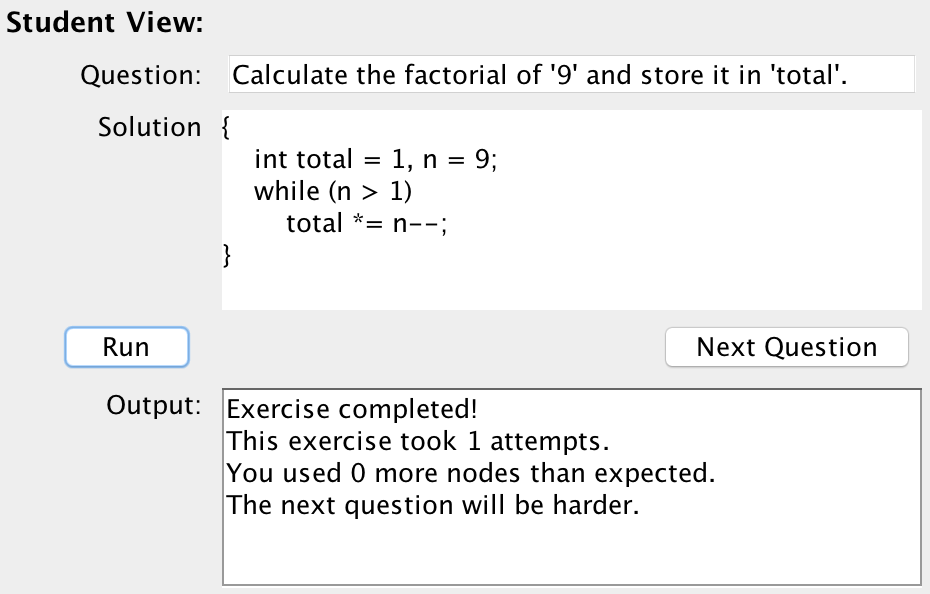
\includegraphics[width=.9\linewidth]{BestSub}
    \caption{The result of solving the question in one attempt and with no extra nodes.}
    \label{SFig:GGS2}
  \end{subfigure}
  \\
  \vspace{5mm}
  \begin{subfigure}{.55\textwidth}
    \centering
    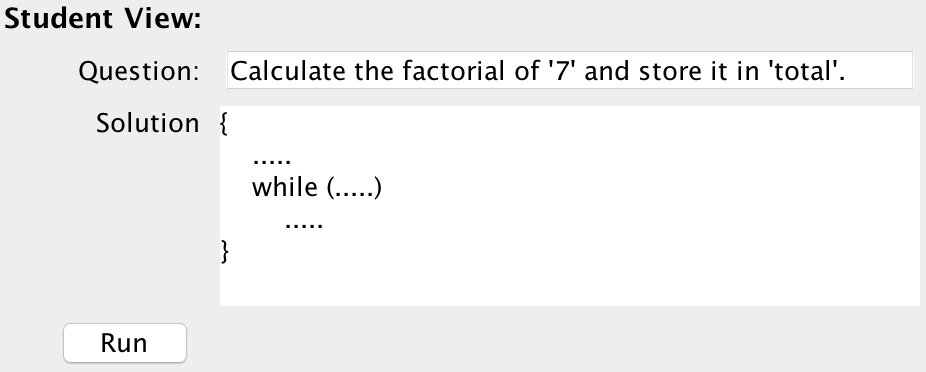
\includegraphics[width=.9\linewidth]{NextQ}
    \caption{The harder question presented next.}
    \label{SFig:GGS3}
  \end{subfigure} 
\caption{Screenshots of the GUI when the student has performed to a standard required for a more difficult exercise.}
\label{Fig:GoodGUIScreens}
\end{figure}

The result of a perfect solution (shown in Figure \ref{SFig:GGS2}) is recorded in the ``Output:'' part of the GUI, which gives feedback on the number of attempts and the number of nodes used, and states that the next question will be harder. This question (shown in Figure \ref{SFig:GGS3}) is presented when the student presses the ``Next Question'' button. While a solution has only one way of being successful, there are a variety of ways in which it can be unsatisfactory. Some possible ways are shown in Figure \ref{Fig:BadGUIScreens}.

\begin{figure}
\centering
  \begin{subfigure}{.6\textwidth}
    \centering
    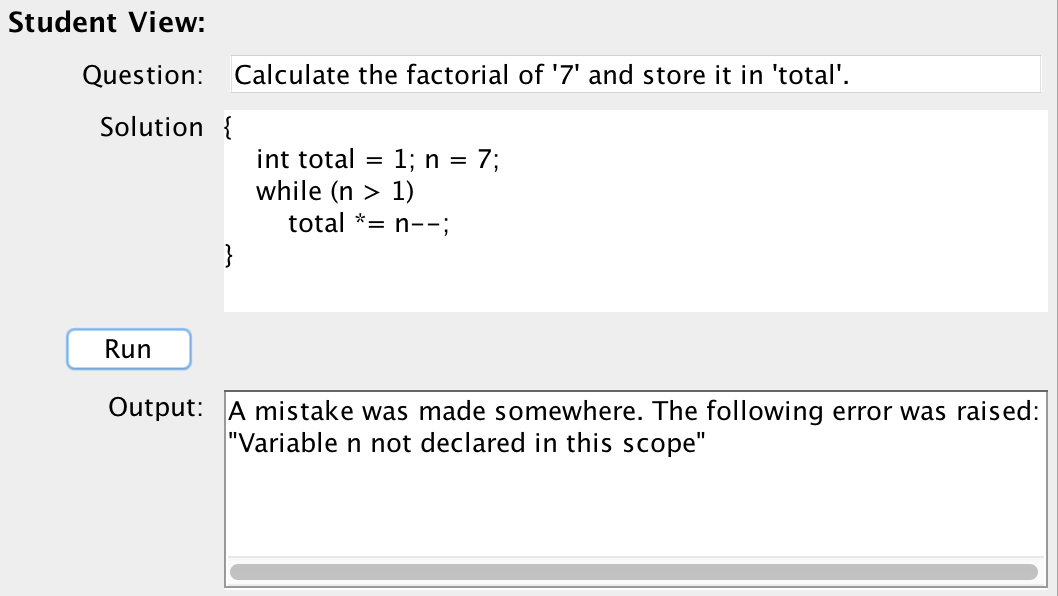
\includegraphics[width=.9\linewidth]{AMistake}
    \caption{The punctuation mark after \texttt{total~=~1} in the first line of the code should be a comma, not a semi-colon. This mistake manifests as the error shown in the ``Output:'' box.}
    \label{SFig:BGS1}
  \end{subfigure}%
  \\
  \vspace{5mm}
  \begin{subfigure}{.45\textwidth}
    \centering
    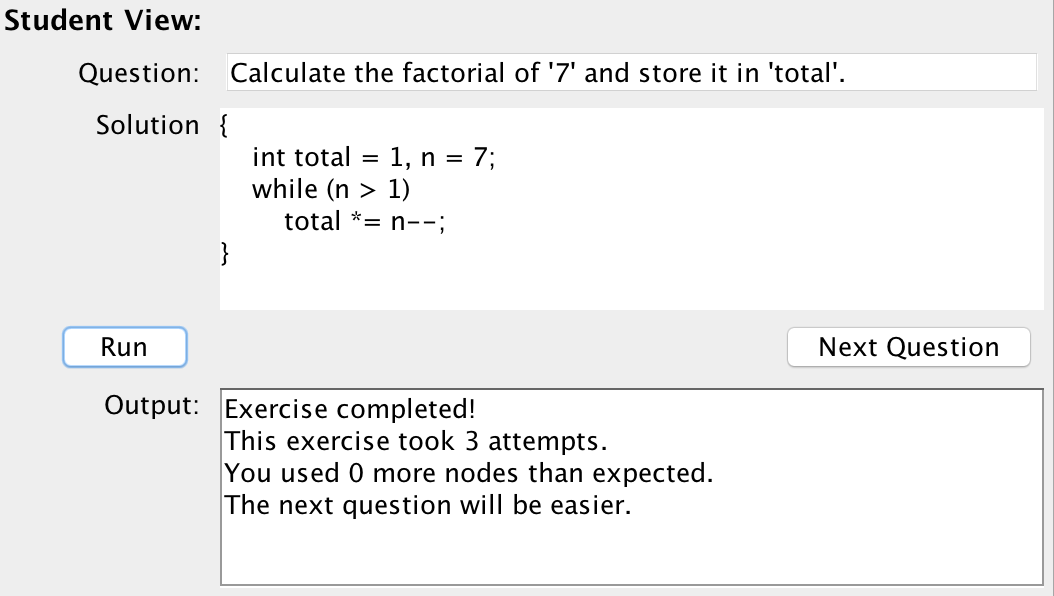
\includegraphics[width=.9\linewidth]{EasierForAttempts}
    \caption{The result of solving the question in more than one attempt.}
    \label{SFig:BGS2}
  \end{subfigure}
  \;
  \begin{subfigure}{.45\textwidth}
    \centering
    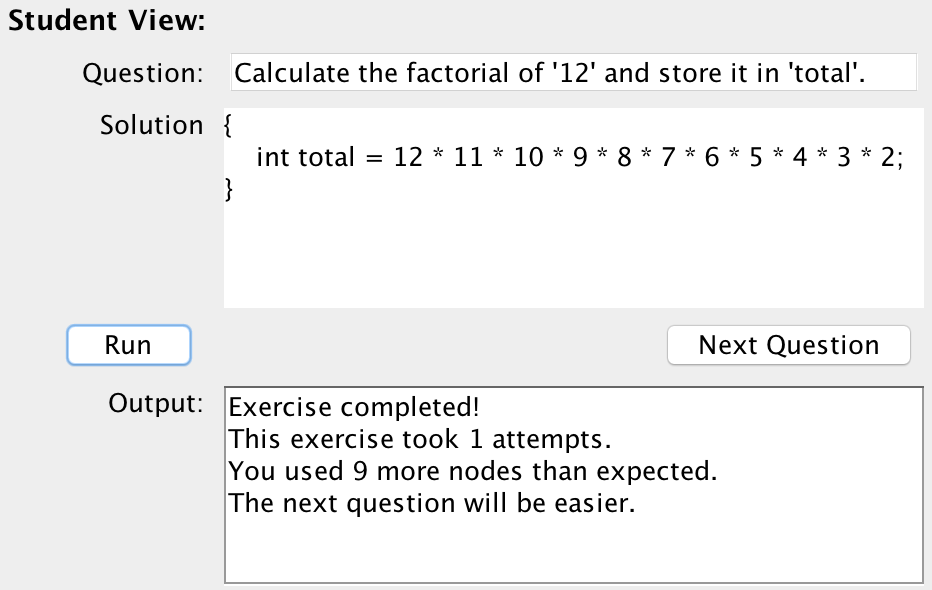
\includegraphics[width=.9\linewidth]{EasierForNodes}
    \caption{The result of solving the question using many more nodes than required.}
    \label{SFig:BGS3}
  \end{subfigure} 
\caption{Screenshots of the GUI when the student's measured performance warrants an easier exercise.}
\label{Fig:BadGUIScreens}
\end{figure}

When a mistake is made, the error thrown by the interpreter is propagated up and shown by the GUI. This enables the student to find the error they made and correct it. A subtle mistake has been made in the code displayed in Figure \ref{SFig:BGS1}. In the first line of the code, the punctuation after the word ``total'' should be a comma, not a semi-colon, to show that ``n = 7'' was part of the local variable declaration, not an assignment. And indeed, the error shown by the GUI tells us that ``The variable n has not been declared". 

For this example, say that the student made another mistake (which is not shown), before finally submitting a correct answer as in Figure \ref{SFig:BGS2}. Since the student took three attempts to solve the exercise, the system determines that the student has not met the standard required for the exercise so, as stated in the ``Output:'' box, the next exercise will be easier. 

Another possible issue a student could have is not understanding how to use the appropriate code construct to attain the most efficient result. This is shown in Figure \ref{SFig:BGS3}, where rather than use a while loop to calculate a factorial they have simply written out the whole long calculation. It is debatable which of the two solutions is preferable in general, but given the purpose of this exercise was to teach how to use while loops, the system is programmed to decide that the given solution was unsatisfactory. This can be seen in the ``Output:'' panel that lists that even though the problem was solved in one attempt, nine more nodes were used than expected, so the next question will be easier.

These figures have demonstrated that the GUI acts as a successful interface between a student and the system, providing a simple way to submit solutions and useful feedback with which a student can evaluate their own performance.

\section{Adjusting the difficulty}
\label{Sec:DiffTrends}

I explained the way that the \texttt{ExerciseSetter} class measured the performance of a student by reference to their correct solution in Section \ref{Sec:ExSetEval}. In this section I explain how the performance measurement is used to determine the difficulty of the following exercise, and the trends that arise from this method.

\begin{figure}
\centering
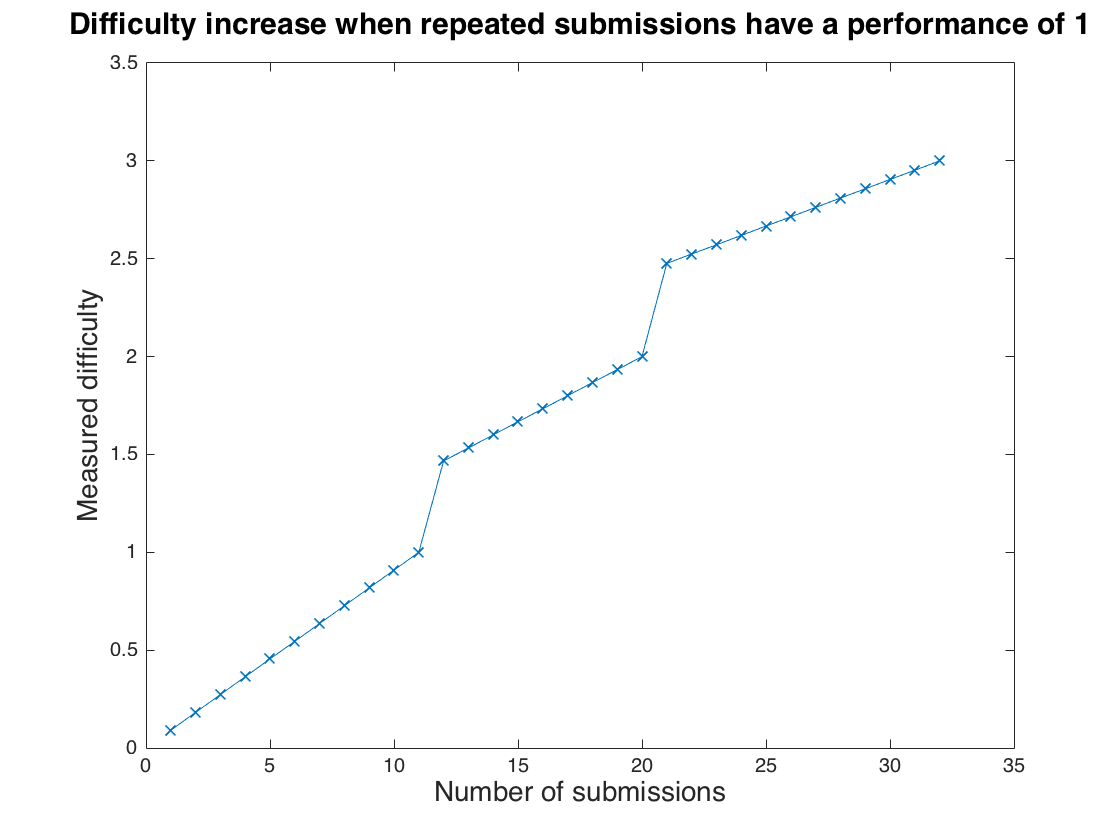
\includegraphics[width = .9\linewidth]{DiffGraph}
\caption{Increase in measured difficulty with repeated submissions each with a measured performance of one.\textcolor{red}{Is this graph meaningful?}}
\label{Fig:DiffGraph}
\end{figure}

Figure \ref{Fig:DiffGraph} shows how the difficulty of the exercises presented by the \texttt{ExerciseSetter} increases as a function of correct solutions submitted. To generate this graph, I determined the difficulty of the exercise being set by the \texttt{ExerciseSetter} to be as low as possible, that is, the simplest question with only a single blank in its model solution. I then submitted a number of correct solutions, tailored such that they all had a measured performance value of one. In practice this is unrealistic, as it corresponds to the student's performance increasing at exactly the same rate as the increase in difficulty. However, as a hypothetical model this can still be instructive. The level of difficulty of each exercise was increased by adding another blank to the model solution until the entire solution was blank. After the final correct submission, the next most difficult question was set.  

At present, there are three questions that the \texttt{ExerciseSetter} can ask which are shown on the graph as three distinct groups of points. The points are separated by small increases in difficulty within questions and a significant increase in difficulty between each of the three questions. The significant increases can be explained by my choice of how the system determines the level of difficulty when a question is presented for the first time. Instead of giving the exercise the lowest difficulty possible (i.e. leaving only a single blank in its model solution), the system sets half of the model solution to be blank. This ensures that when a student attempts a problem for the first time they are not provided with the majority of the code.

For the three questions illustrated, there is a tendency for the model solution to require more nodes to solve the problem when the question is more complex. This has the unintended effect of making the rate of increase in difficulty slower as the difficulty of the question itself increases. This can be seen more explicitly in Figure \ref{Fig:DiffGraphComp}, where each solid line corresponds to a single question. It will be noted that the gradient of these lines decreases as the questions get more complex as does the increase in difficulty as a function of a correct solution. This is desirable as students are likely to require smaller increments in difficulty as the questions get more complex. Although this tendency may not hold for all questions (i.e. there may be some simple questions that require a lot of nodes to answer, and some complex ones that can be solved with very few nodes), I believe that it will hold for a large number of questions, making this a useful side effect of my particular implementation.

\begin{figure}
\centering
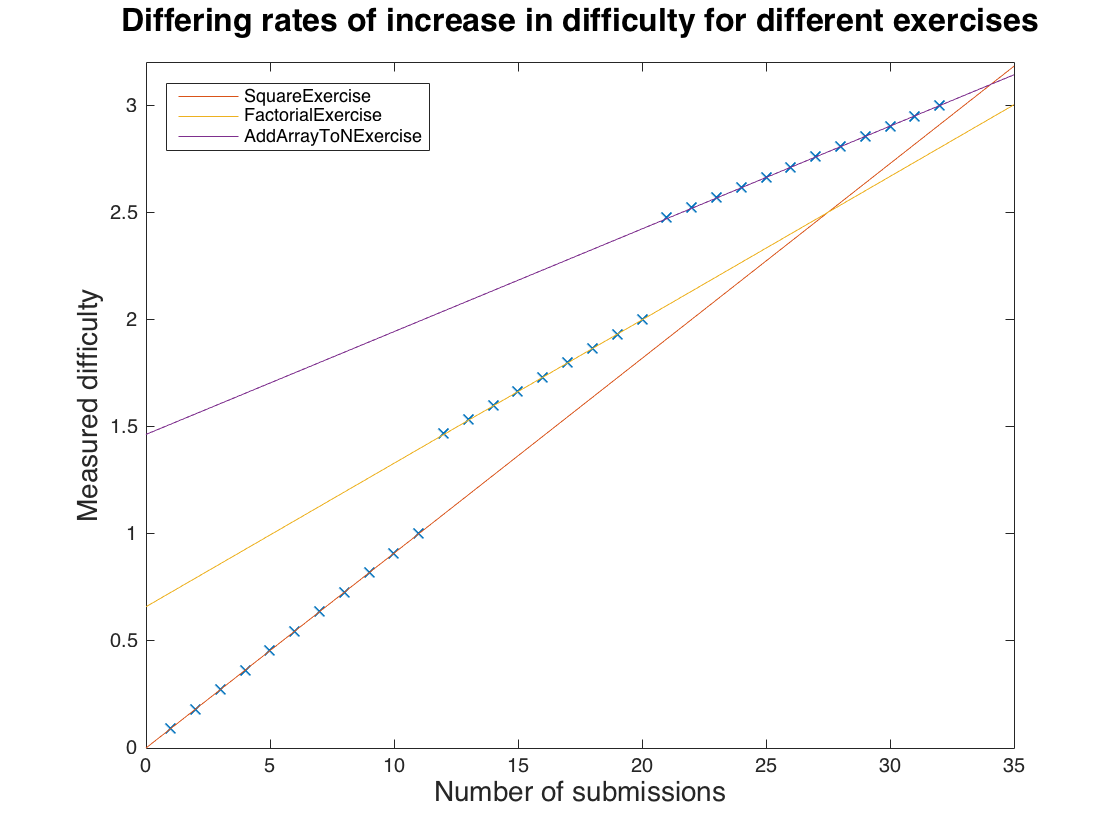
\includegraphics[width = .9\linewidth]{DiffGraphComp}
\caption{This demonstrates the different rates of increase of difficulty found for the different questions. The straight lines are extrapolated past the original points to show that they intersect and thus are not parallel.}
\label{Fig:DiffGraphComp}
\end{figure}

In this section I have described the trends present in the way difficulty is modified according to a student's performance.

\section{Development process}
\label{Sec:DevProc}

Throughout the implementation process, I followed the principles of Test Driven Development (TDD)\footnote{http://agiledata.org/essays/tdd.html - last accessed 10th May}. This methodology revolves around the writing of unit tests before the appropriate code is written. These tests are designed with reference to the requirements specification, such that any software that passes these tests fulfils the requirements. I found it very useful to develop the software in this manner, since I found that most bugs that I introduced were caught the first time I executed the code, and thus could not cause more problems later in the process, when they might have been harder to find.

The development of prototypes has also been beneficial, allowing me to avoid dead ends by testing my ideas at an early stage. However, at times I might have benefited from determining the interfaces between the components before I started to make prototypes of them. Sometimes the prototypes became the components themselves, and it was only when I tried to get them to work together that I realised that the interface one component expected was not necessarily the one that another component offered. In future, I would outline the project not only in text form, but also as a UML diagram.

I recognise that a limitation of the project is that my evaluation has relied on the system itself, without using an external metric of quality. Such a metric might be attained by asking a sample of students with varying ages, experience, and competence in programming to evaluate their own performance at solving these questions and comparing this with my system's measurement of their performance.

%%%%%%%%%%%%%%%%%%%%%%%%%%%%%%%%%%%%%%%%%%%%%%%%%%%%%%%%%%%%%%%%%%%%%
% Conclusion Chapter

\chapter{Conclusion}

In conclusion the project was a success, as the software I developed fulfils all of the original aims. Furthermore, I was able to implement two extensions on top of the core functionality that have enabled me to demonstrate the power of the underlying system.

I have designed a new language, MiniJava, such that its programs can incorporate blanks that must be filled in before they can be executed. I have written an interpreter and a pretty-printer for this language, to execute arbitrary code and print representations of programs as MiniJava code. I encoded a representation of programming exercises and wrote algorithms to introduce blanks to and remove them from the model solutions for these exercises, making them harder and easier respectively. Using concrete examples of such exercises I implemented a system that delivers questions to a student, allows them to fill in the blanks with their own arbitrary code, and executes the completed code to determine whether the problem was solved. This system measures the performance of the student using a heuristic and adjusts the difficulty of the next exercise based on this measurement. As extensions, I implemented a parser for MiniJava to streamline the process of accepting student input, and created a GUI to demonstrate how both teachers and students might use the system.

This project has several limitations. The choices I made regarding pedagogic practice were based on my experience as a learner and teaching assistant in a variety of settings. With hindsight it would have been useful to include more pedagogical theory in the preparation phase to inform these choices. A further limitation is that the system has a limited number of questions that may be set which means that the system needs to present the same question multiple times. This means that currently it is possible for students to simply learn the answers through repetition of the material without actually understanding the underlying principles. 

\section{Further work}

MiniJava is only a subset of the full Java grammar. Since it is Java that students need to learn, adding the rest of Java's features to MiniJava would be worthwhile to enable the system to be used at a higher level. Currently this system would be useful for students who are beginning to learn Java as they only need to understand the features present in MiniJava, but it wouldn't be useful for a student who needs to learn more complex principles such as how to write functions and classes.

One of the difficulties in teaching programming is that it is often difficult to report errors in a way that novice programmers find useful. Often these errors are presented using technical jargon that beginners may not have learnt, and usually require a deeper understanding of the language (and Computer Science in general) than can be expected of them. One tool that has made some headway in solving this problem is Arjen \cite{Arjen}. This works by exploiting the fact that novice programmers all tend to make the same types of errors and explicitly searches for these errors in order to provide feedback tailored to a novice, perhaps giving pointers for how to solve or avoid the problem. Since Arjen takes a Java source file as input it is feasible that students' MiniJava solutions could be passed to the tool as code before they are parsed, especially if the rest of Java's features have been implemented. The reports generated by Arjen could then be passed back to the student, giving them better explanations of their mistakes. Such a collaboration would be likely to provide a much more supportive user experience for novice programmers.

Another extension I considered in my proposal but did not have time to implement was to consider different syntactic constructs separately and attempt to record a student's expertise with each construct. This means that when students use a specific syntax construct (e.g. a \texttt{for} loop) the system could assess and record whether a student understands how to use that construct. The system could then focus attention on areas that a student had demonstrated less comprehension of, enabling it to provide a more tailored and directed learning experience.\\

In summary, this project has been both a useful insight into the development of complex software in general, and also a successful implementation of a system for giving programming exercises adaptive difficulty.

%%%%%%%%%%%%%%%%%%%%%%%%%%%%%%%%%%%%%%%%%%%%%%%%%%%%%%%%%%%%%%%%%%%%%
% the bibliography
\addcontentsline{toc}{chapter}{Bibliography}
\bibliography{refs}

%%%%%%%%%%%%%%%%%%%%%%%%%%%%%%%%%%%%%%%%%%%%%%%%%%%%%%%%%%%%%%%%%%%%%
% the appendices
\appendix

\chapter{The Grammar}
\label{App:Parser}

\begin{Verbatim}[tabsize=4]
grammar MiniJava;

// STATEMENTS / BLOCKS

// entry point
entry
	: block [true]			# blockEntry
	| blockStatement+		 # blockStatementsEntry
	| statementTop			# statementEntry
	| expression			  # expressionEntry
	;									

block [boolean isOuter]
	: LBRACE blockStatement* RBRACE						
	;

blockStatement
	: primitiveType variableDeclarators SEMI	# localVariableDeclaration
	| statement								 # makeStmnt
	| variableDeclarator					    # makeVarDec
	;
    
statementTop
	: statement					   # stmnt
	| statementNSI					# stmntNSI
	;

\end{Verbatim}
\begin{Verbatim}[samepage=true, tabsize=4]
statement
	: block [false]									 # makeBlock
	| IF parExpression statement 					   # makeIf
	| IF parExpression statementNSI ELSE statement	  # makeITE
	| FOR LPAREN forInit? SEMI expression? 
		SEMI expressionList? RPAREN  statement		  # makeFor
	| WHILE parExpression statement					 # makeWhile
	| statementNTS									  # makeStatementNTS
	;
\end{Verbatim}

\begin{Verbatim}[tabsize=4]  
statementNSI
	: block [false]									  # makeBlockNSI
	| IF parExpression statementNSI ELSE statementNSI	# makeITENSI
	| FOR LPAREN forInit? SEMI expression? 
		SEMI expressionList? RPAREN statementNSI 		# makeForNSI
	| WHILE parExpression statementNSI				   # makeWhileNSI
	| statementNTS									   # makeStatementNTSNSI												
	;
    
statementNTS
	: DO statement WHILE parExpression SEMI	  # makeDo
	| RETURN SEMI								# return
	| BREAK SEMI								 # break
	| CONTINUE SEMI							  # continue
	| SEMI									   # empty
	| expressionStatement SEMI				   # makeStmntExpr
	;


forInit
	: primitiveType variableDeclarators			 # forInitLVD
	| expressionList								# forInitExprs
	;

// EXPRESSIONS

parExpression
	: LPAREN expression RPAREN
	;

expressionList
	: expression (COMMA expression)*
	;

expressionStatement
	: expression
	;

expression // Most binding comes first!
	: Identifier											   # makeID
	| expression LBRACK expression RBRACK					  # arrayAccess
	| parExpression										    # makeBracketed
	| literal												  # makeLiteral
	| expression (op=INC | op=DEC)							 # postInc
	| (op=ADD|op=SUB|op=INC|op=DEC) expression				 # preIncEtc
	| BANG expression										  # makeNot
	| expression (op=MUL|op=DIV) expression				    # multExpr
	| expression (op=ADD|op=SUB) expression			  	  # addExpr
	| expression (op=LE | op=GE | op=GT | op=LT) expression	# relationalExpr
	| expression (op=EQUAL | op=NOTEQUAL) expression		   # eqExpr
	| expression AND expression								# andExpr
	| expression OR expression								 # orExpr
	| <assoc=right> expression QUESTION 
		expression COLON expression						    # condExpr
	| <assoc=right> expression												
		(   op=ASSIGN
        		|   op=ADD_ASSIGN
        		|   op=SUB_ASSIGN
        		|   op=MUL_ASSIGN
        		|   op=DIV_ASSIGN
        		)
        		expression									 # assignExpr
	;
    
// VARIABLES AND LITERALS
    
variableDeclarators
	: variableDeclarator (COMMA variableDeclarator)*
	;

variableDeclarator
	: Identifier LBRACK RBRACK (ASSIGN variableInitializer)?   # arrayVarDec 
	| Identifier (ASSIGN variableInitializer)?				 # singleVarDec
	;
\end{Verbatim}
\begin{Verbatim}[samepage=true,tabsize=4]
variableInitializer 
	: arrayInitializerValues								   # arrayInitVals
	| arrayInitializerSize									 # arrayInitSize
	| expression											   # initExpr
	;
\end{Verbatim}
\begin{Verbatim}[tabsize=4]
arrayInitializerValues
	: LBRACE variableInitializer (COMMA variableInitializer)* (COMMA)? RBRACE	
	;
    
arrayInitializerSize
	: NEW primitiveType LBRACK expression RBRACK
	;

primitiveType
	: BOOLEAN
	| CHAR
	| INT
	| DOUBLE
	;

literal
	: IntegerLiteral 
	| FloatingPointLiteral 
	| CharacterLiteral
	| BooleanLiteral
	;

// LEXER
// �3.9 Keywords

BOOLEAN	    : 'boolean';
BREAK		  : 'break';
CHAR		   : 'char';
CONTINUE	   : 'continue';
DO			 : 'do';
DOUBLE		 : 'double';
ELSE		   : 'else';
FOR			: 'for';
IF			 : 'if';
INT			: 'int';
NEW			: 'new';
RETURN		 : 'return';
WHILE		  : 'while';

// �3.10.1 Integer Literals
// �3.10.2 Floating-Point Literals
// �3.10.3 Boolean Literals
// �3.10.4 Character Literals
// �3.11 Separators
// Sections removed for clarity

LPAREN          : '(';
RPAREN          : ')';
LBRACE          : '{';
RBRACE          : '}';
LBRACK          : '[';
RBRACK          : ']';
SEMI            : ';';
COMMA           : ',';
DOT             : '.';

// �3.12 Operators

ASSIGN          : '=';
GT              : '>';
LT              : '<';
BANG            : '!';
QUESTION        : '?';
COLON           : ':';
EQUAL           : '==';
LE              : '<=';
GE              : '>=';
NOTEQUAL        : '!=';
AND             : '&&';
OR              : '||';
INC             : '++';
DEC             : '--';
ADD             : '+';
SUB             : '-';
MUL             : '*';
DIV             : '/';

ADD_ASSIGN      : '+=';
SUB_ASSIGN      : '-=';
MUL_ASSIGN      : '*=';
DIV_ASSIGN      : '/=';

// �3.8 Identifiers (must appear after all keywords in the grammar)
//
// Whitespace and comments
//
// Sections removed for clarity
\end{Verbatim}

\chapter{Project Proposal}

% Note: this file can be compiled on its own, but is also included by
% diss.tex (using the docmute.sty package to ignore the preamble)
\documentclass[12pt,a4paper,twoside]{article}
\usepackage[pdfborder={0 0 0}]{hyperref}
\usepackage[margin=25mm]{geometry}
\usepackage{graphicx}
\usepackage{parskip}
\begin{document}

\begin{center}
\Large
Computer Science Tripos -- Part II -- Project Proposal\\[4mm]
\LARGE
A System for Giving Programming Exercises \\Adaptive Difficulty\\[4mm]

\large
R.~J.~McFarland, Homerton College

Originator: M.~B.~Gale

20 October 2016
\end{center}

\vspace{5mm}

\textbf{Project Supervisor:} M.~B.~Gale

\textbf{Director of Studies:} Dr J.~Fawcett

\textbf{Project Overseers:} Dr D.~J.~Greaves  \& Prof J.~G.~Daugman

% Main document

\section*{Introduction}

Different people learn at different speeds, and learn some things more quickly than others. When a group of students are given a set of programming exercises, this typically isn't taken account of. The aim of this project is to design a system that varies the difficulty of a programming exercise depending on how the individual has performed completing previous exercises. 

The difficulty of an exercise can be measured using two metrics: how complex the problem being solved is and how much code the student is expected to write. The system will vary both of these to adapt the difficulty of proposed exercises automatically (i.e. the system will not look for preprogrammed mistakes, but rather interpret the mistakes made and react accordingly). When an exercise is completed to a sufficient standard, a similar exercise will be given, but expecting more code to be written. When the system has determined that the problem has been mastered, a more difficult problem will be presented, requiring less code to be written again.

\section*{Resources required}

I shall use my own Macintosh laptop for the majority of this project. Backup will be to GitHub and to a 5TB hard drive I keep in my room. I shall make use of the Java standard library, as well as the JavaFX library for the graphical user interface element. I require no special resources.

\section*{Starting point}

I am able to program in Java, and have used JavaFX before for the Part IB group project. During my A-Levels I wrote a program to test the maths abilities of Year 4 students, which involved the programmatic generation of various kinds of maths questions.

\section*{Work to be done}

The work for this project can be split up into the following sub-projects:
\begin{enumerate}
\item{A representation of a programming exercise must be coded up to allow the final product to manipulate them.}
\item{A heuristic that measures the difficulty of a given exercise must be chosen and implemented.}
\item{A heuristic that assesses how well a ``student'' has completed an exercise must be chosen and implemented.}
\item{I must devise a system, using the previous three items, that determines which exercise should be given to the student next, as well as how much of the required code is already filled in, based on the student's performance completing previous exercises.}
\item{A Graphical User Interface should be designed to enable a user to manually adjust the content of a given programming exercise.}
\item{In order to test the program, a student will be simulated by creating a system that tells the program what errors were made where and how long the exercise took to be solved, so that the program's response to various stimuli can be measured.}
\end{enumerate}

\section*{Success Criteria}

The project will be considered completed when:
\begin{enumerate}
\item{I have a system that presents the same initial problem to all students.}
\item{The system can determine that code written by the student solves the given problem.}
\item{On registering completion of the exercise, the system will then present a new problem to the student.}
\item{If the student solved this problem with sufficient ease as measured by my performance heuristic, then this new problem will be more difficult, as measured by my difficulty heuristic.}
\item{If the student failed to solve the problem, or took too much time or made too many errors, then the next problem will be easier.}
\item{The system will adjust the difficulty of a given problem in line with the difficulty heuristic by changing the amount of code required to solve the problem, and also the underlying problem being solved.}
\end{enumerate}

\section*{Possible extensions}

\begin{itemize}
\item{This system could be improved such that it identifies which concepts a student is struggling with and adjusts the content of future exercises to encourage learning of these concepts.}
\item{The program could produce a graph of progress against time to motivate learners.}
\item{A simple game that utilises this system could be made, to showcase how the system might be used to teach programming.}
\end{itemize}

\section*{Timetable}

\textbf{24th Oct - 6th Nov:} 
\begin{itemize}
\item{Research adaptive difficulty and see how it has been done before.}
\item{Research how errors in code have been quantified in the past.}
\item{Research where and how simulated users have been designed to test systems.}
\end{itemize}

\textbf{7th Nov - 20th Nov:}
\begin{itemize}
\item{Describe how code that solves an exercise could be split up into discrete sections, and a way to store how well each of those sections was completed.}
\end{itemize}
\underline{Milestones:}
\begin{itemize}
\item{Have a representation of a programming puzzle in Java code.}
\end{itemize}

\textbf{21st Nov - 4th Dec:}
\begin{itemize}
\item{Prototype and compare heuristics to measure the ``difficulty'' of a given programming exercise, based on the difficulty of the goal to be achieved, and how much of the code is presented initially.}
\end{itemize}
\underline{Milestones:}
\begin{itemize}
\item{Select and implement a difficulty heuristic.}
\end{itemize}

\textbf{5th Dec - 18th Dec:}
\begin{itemize}
\item{Prototype and compare heuristics to measure performance, based perhaps on how much time was taken, the number of errors made and the time the solution takes to run.}
\end{itemize}
\underline{Milestones:}
\begin{itemize}
\item{Select and implement a performance heuristic.}
\end{itemize}

\textbf{19th Dec - 1st Jan:}
\begin{itemize}
\item{Slack time over Christmas to catch up if I need to.}
\end{itemize}

\textbf{2nd Jan - 15th Jan:}
\begin{itemize}
\item{Implement a system to adapt the difficulty of the programming exercises by presenting a new, more difficult problem each time an exercise is completed satisfactorily, and presenting an easier one if the student is struggling too much.}
\end{itemize}
\underline{Milestones:}
\begin{itemize}
\item{Have a system that will present a problem to a student, determine that the student has solved the problem with the code they have written, determine if the student found it too easy or too hard, and present the student with a new problem that is either easier or harder respectively.}
\end{itemize}

\textbf{16th Jan - 29th Jan:}
\begin{itemize}
\item{Write Progress Report.}
\item{Improve the system by implementing the concept of changing the amount of code that needs to be written to solve a given problem as another way of affecting its difficulty.}
\end{itemize}
\underline{Milestones:}
\begin{itemize}
\item{Have the system extended such that it may require the student to write more or less code to make more fine grained adjustments to the difficulty of a programming problem.}
\end{itemize}

\textbf{30th Jan - 19th Feb:}
\begin{itemize}
\item{\textbf{3rd Feb:} Submit the Progress Report}
\item{Design a user interface to change the content of the programming exercise to be solved.}
\end{itemize}
\underline{Milestones:}
\begin{itemize}
\item{Have a user interface with controls to determine the exact difficulty of the problem about to be presented.}
\end{itemize}

\textbf{20th Feb - 5th Mar:}
\begin{itemize}
\item{Write unit tests for all units.}
\end{itemize}
\underline{Milestones:}
\begin{itemize}
\item{Have unit tests written for every unit of the code.}
\end{itemize}

\textbf{6th Mar - 19th Mar:}
\begin{itemize}
\item{Test the implementation by simulating a student ``using'' the system by ``solving'' problems with varying success.}
\end{itemize}
\underline{Milestones:}
\begin{itemize}
\item{Have a simulated student that will tell the system what mistakes were made in the code and where, as well as how long it took to solve the problem (along with any other parameters deemed important to measuring the performance of the student), such that the response of my system can be measured against the performance of a student using it.}
\end{itemize}

\textbf{20th Mar - 2nd Apr:}
\begin{itemize}
\item{Slack time for catching up and doing extensions.}
\end{itemize}

\textbf{3rd Apr - 16th Apr:}
\begin{itemize}
\item{Write Introduction and Conclusion (about 2,500 words).}
\item{Write up Proforma (excluding word count), Declaration of Originality, Project Proposal and Cover Sheet.}
\end{itemize}
\underline{Milestones:}
\begin{itemize}
\item{Have the above sections of the dissertation written in draft form.}
\end{itemize}


\textbf{17th Apr - 30th Apr}
\begin{itemize}
\item{Write Preparation and Implementation (about 5000 words).}
\end{itemize}
\underline{Milestones:}
\begin{itemize}
\item{Have the above sections of the dissertation written in draft form.}
\end{itemize}

\textbf{1st May - 14th May}
\begin{itemize}
\item{Write Evaluation (about 2500 words).}
\item{Write Contents Page, finish Bibliography, Appendices and Index as required.}
\item{Fill in word count of Proforma.}
\item{Submit draft to DoS and Supervisor.}
\end{itemize}
\underline{Milestones:}
\begin{itemize}
\item{Have the above sections of the dissertation written in draft form.}
\end{itemize}

\textbf{15th May - 19th May}
\begin{itemize}
\item{Incorporate feedback into dissertation.}
\item{\textbf{19th May:} Submit dissertation.}
\end{itemize}


\end{document}

\end{document}
